% !TEX root = main.tex
\section{Acceptance}
\label{sec:Acceptance}

\subsection{MC corrections}

\subsubsection{Truth matching of simulated candidates}

We use the \textsf{BackgroundCategory} tool to truth match our simulated candidates. 
Candidates with background category (\textsf{BKGCAT}) 20 or 50 are considered to be true signal. 
Background category 60 is more peculiar since it contains both badly reconstructed
signal candidates and ghost background.
This is due to the fact that the classification algorithms identifies all tracks 
for which less than $70\%$ of the reconstructed hits are matched to generated truth-level quantities as ghosts.
In particular for signal decays involving many tracks (as in our case),
this arbitrary cutoff is not $100\%$ efficient.
Moreover, the efficiency is expected to depend on the kinematics which would lead to a biased acceptance determination
if candidates with \textsf{BKGCAT}$=60$ would be removed. 
We therefore include \textsf{BKGCAT}$=60$ and statistically subtract the ghost background by using the \textsf{sPlot} technique.
The \textsf{sWeights} are calculated from a fit to the reconstructed $B_s$ mass.  
The signal contribution is modeled as described in Sec.~\ref{subsec:signalModel} and the background with a polynomial.
The fit is performed simultaneously in two categories; the first includes events with \textsf{BKGCAT} = 20 or 50 and
the second events with \textsf{BKGCAT}  = 60.
To account for the different mass resolution we use a different $\sigma$ for each category,
while the mean and the tail parameters are shared between them. 
The background component is only included for the second category.

A significant fraction of $7\%$ of the true signal candidates are classified as ghosts,
while only $20 \%$ of the events classified with \textsf{BKGCAT}$=60$ are indeed genuine ghosts.
%We repeat the efficiency determination with an alternative fit model to assign a systematic uncertainty.


\begin{figure}[h]
\centering
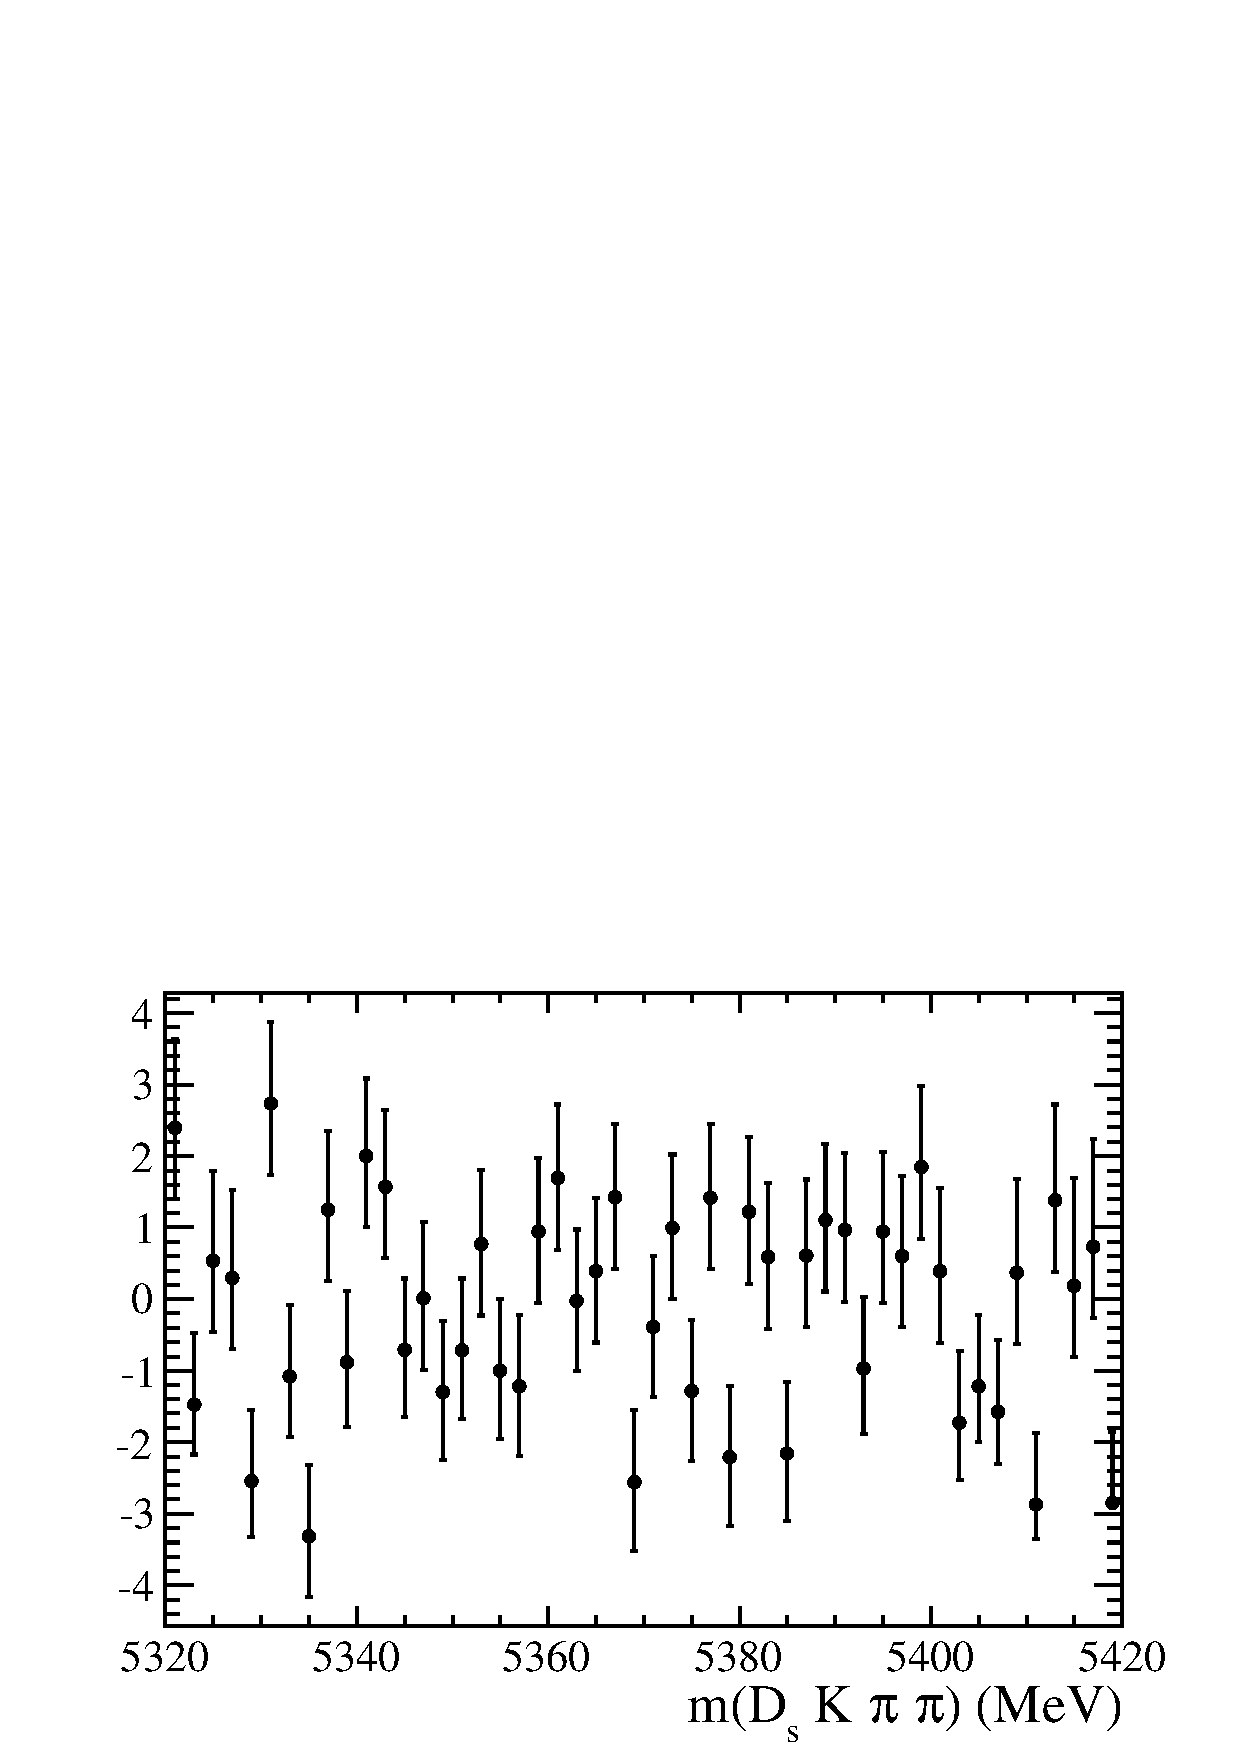
\includegraphics[height=!,width=0.35\textwidth]{figs/MassFit/signalMC_pull.pdf}
\includegraphics[height=!,width=0.35\textwidth]{figs/MassFit/signalMC_ghost_pull.pdf}

%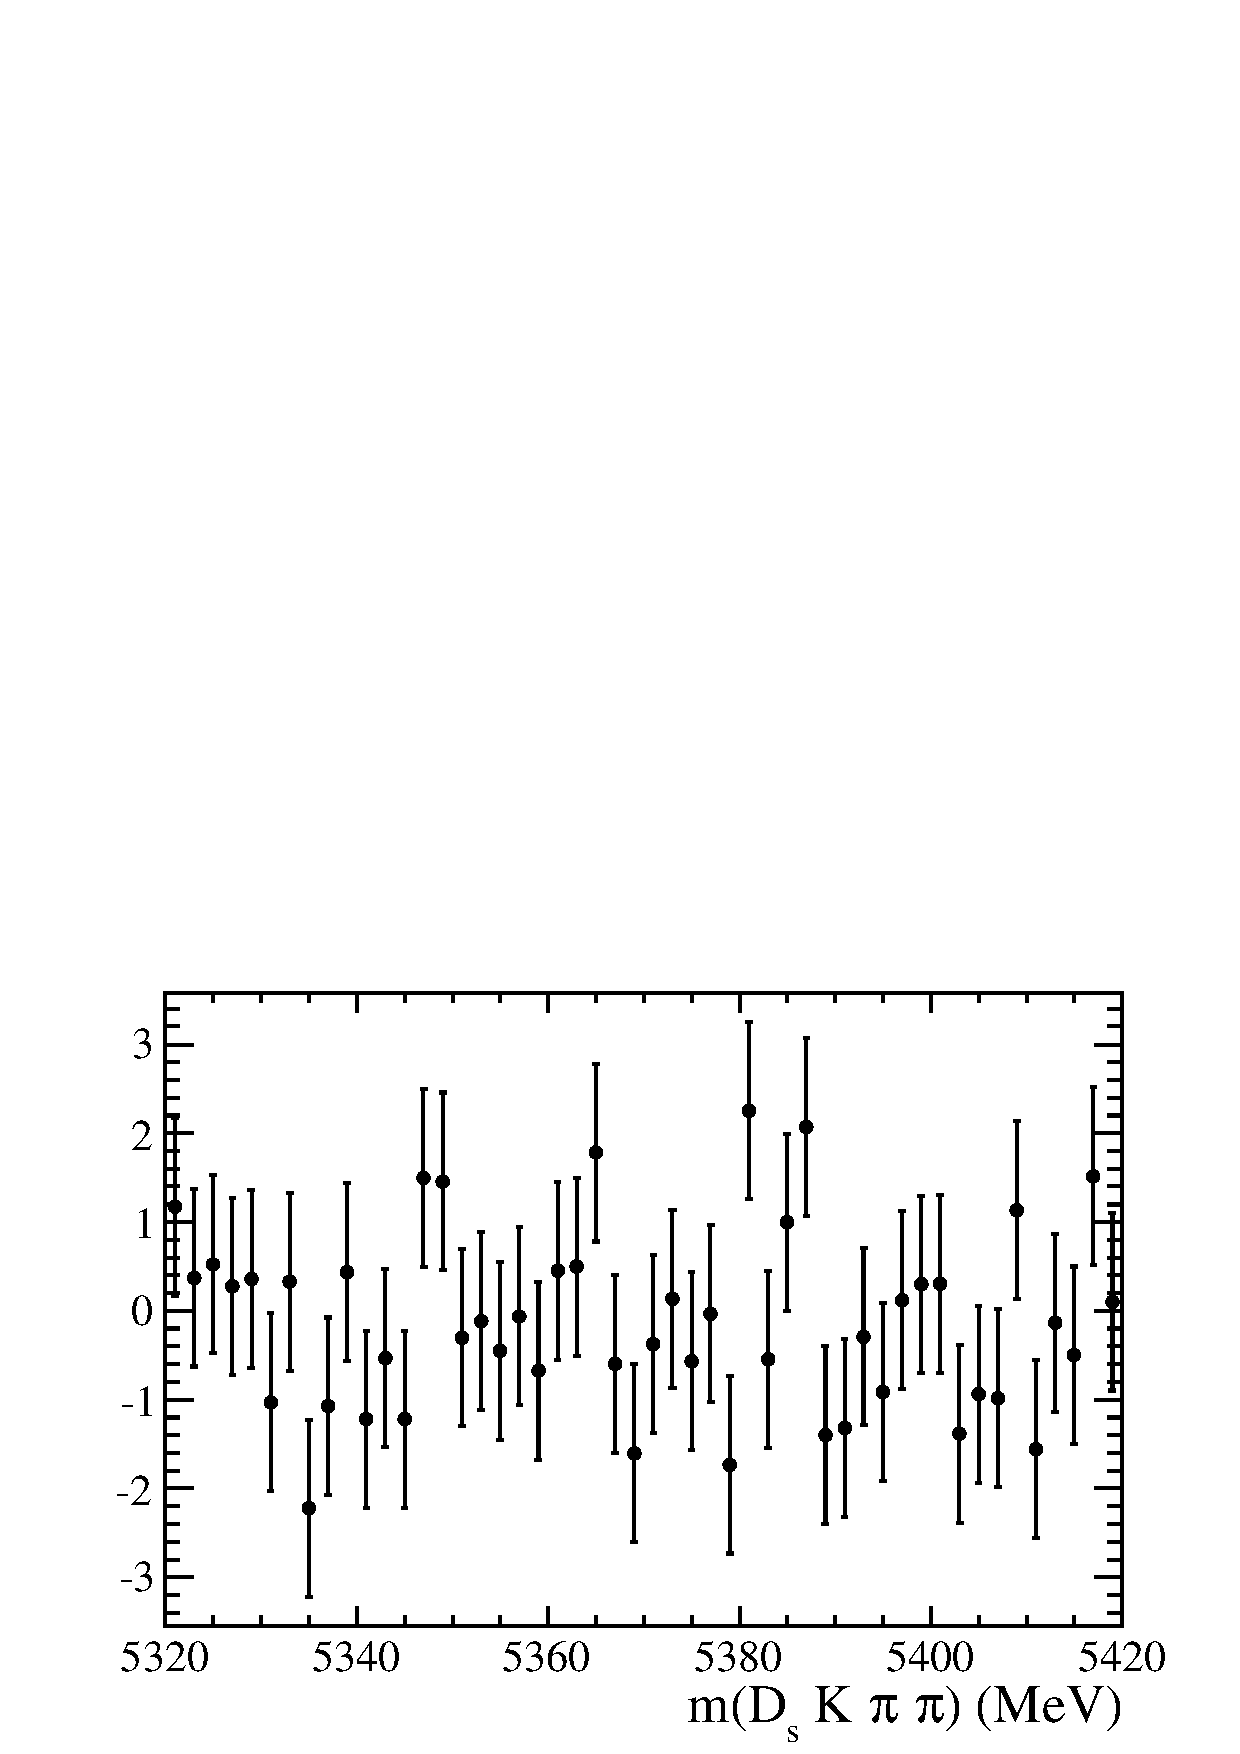
\includegraphics[height=!,width=0.4\textwidth]{figs/MassFit/normMC_pull.pdf}
%\includegraphics[height=!,width=0.4\textwidth]{figs/MassFit/normMC_ghost_pull.pdf}

\caption{\small The reconstructed $B_s$ mass distribution for simulated $B_s \to D_s K \pi \pi$  %(top) and $B_s \to D_s \pi \pi \pi$ (bottom) 
decays classified with \textsf{BKGCAT} = 20 or 50 (left) and \textsf{BKGCAT} = 60 (right) after the full selection. }
\label{fig:}
\end{figure}


\subsubsection{Correction of data-simulation differences}

For the evaluation of phase space efficiency and to a lesser extend also the decay-time efficiency we rely on simulated data 
as discussed in the following sections.
A number of data-driven corrections are applied to the MC samples to account for known data-simulation differences.
The MC sample is reweighted to match the three-dimensional $p_T$, $\eta$ and track multiplicity distribution observed on real data.
%An additional reweighting of the track multiplicity is applied on top of that.
These corrections are derived from the calibration channel $B_s\to D_s \pi\pi\pi$ and applied to both the signal and calibration channel MC samples.
The distributions before and after reweighting are shown in Appendix \ref{a:DataMC}.
We use the \textsf{PIDCorr} tool to correct the simulated PID responses based on PID calibration samples \cite{LHCb-INT-2017-007}.

%\clearpage
%\subsubsection{PID efficiencies}
%
%\begin{figure}[h]
%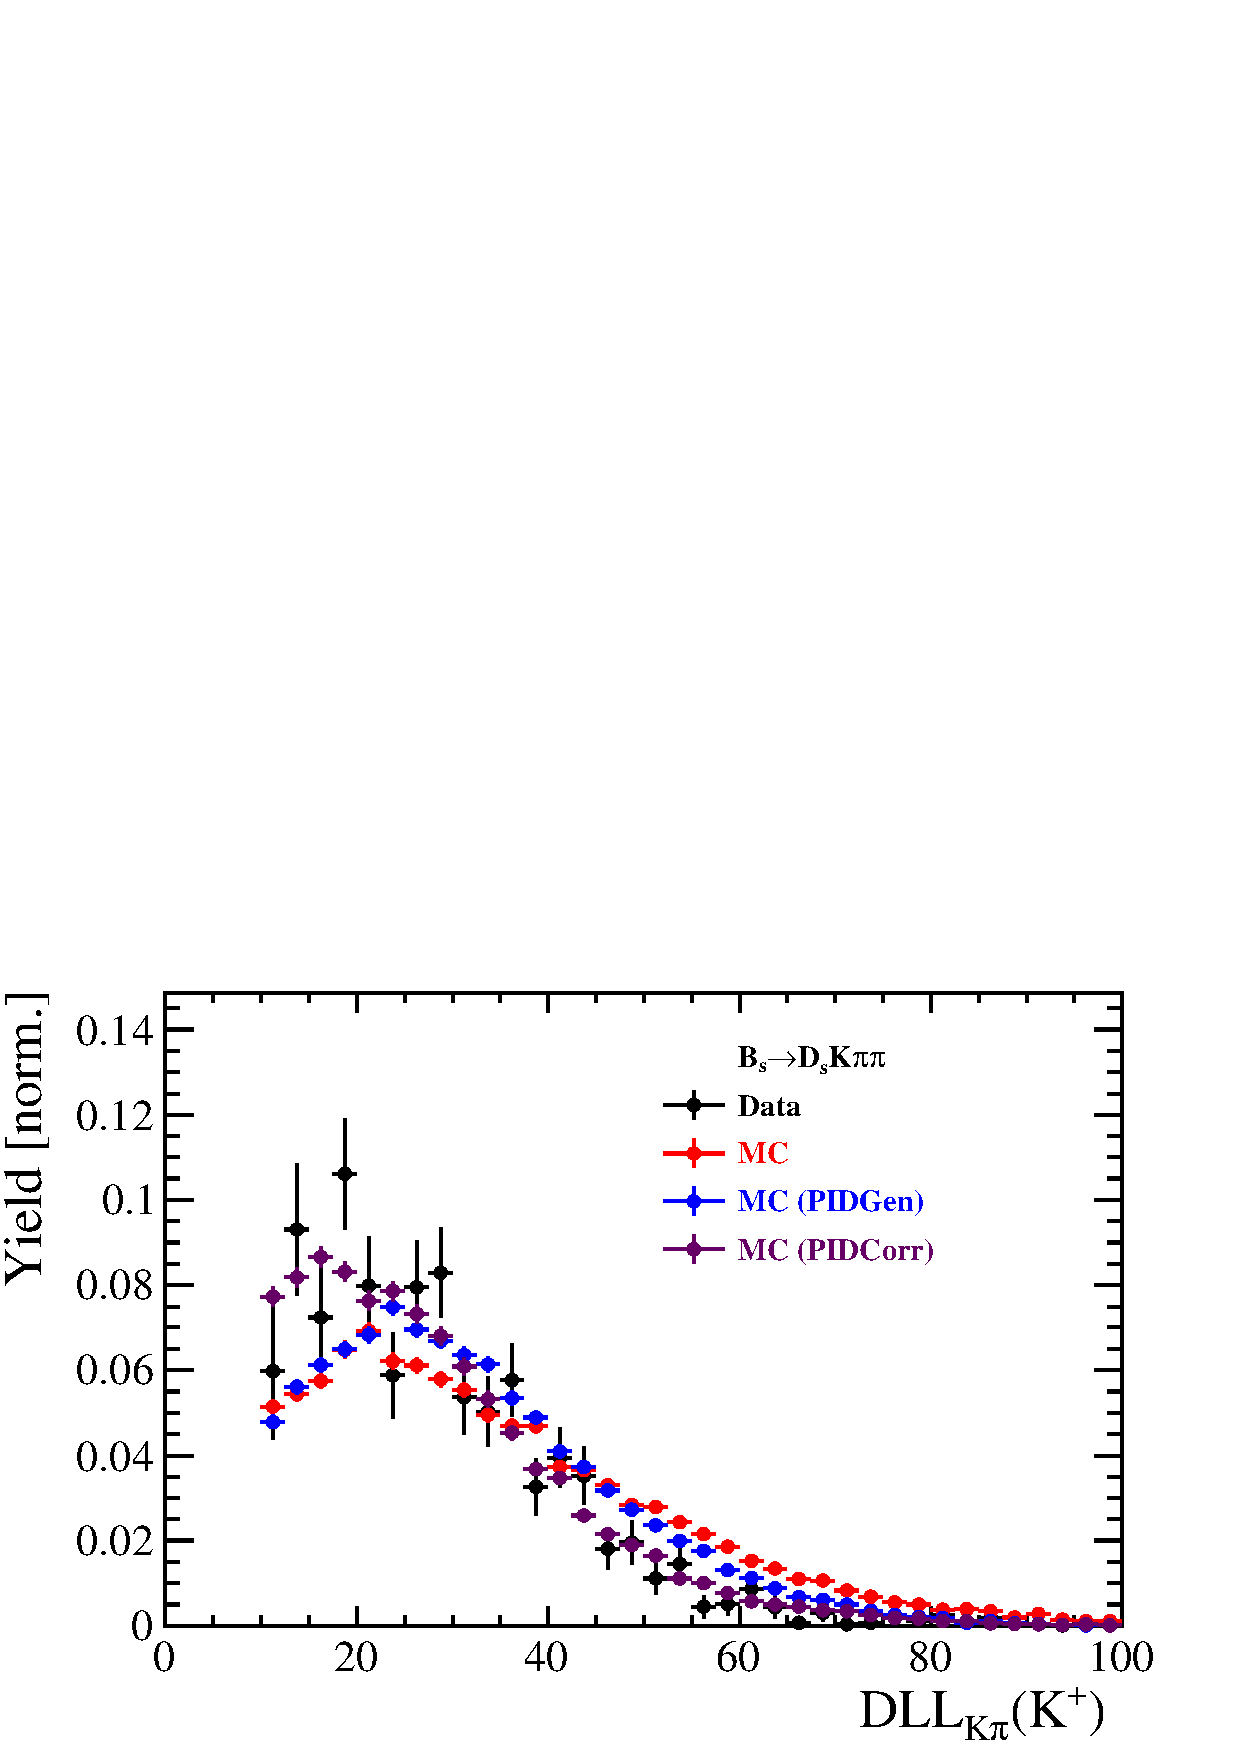
\includegraphics[height=!,width=0.32\textwidth]{figs/dataVsMC/signal_pid/PID_Ds2KKpi_1_K_plus_PIDK.pdf}
%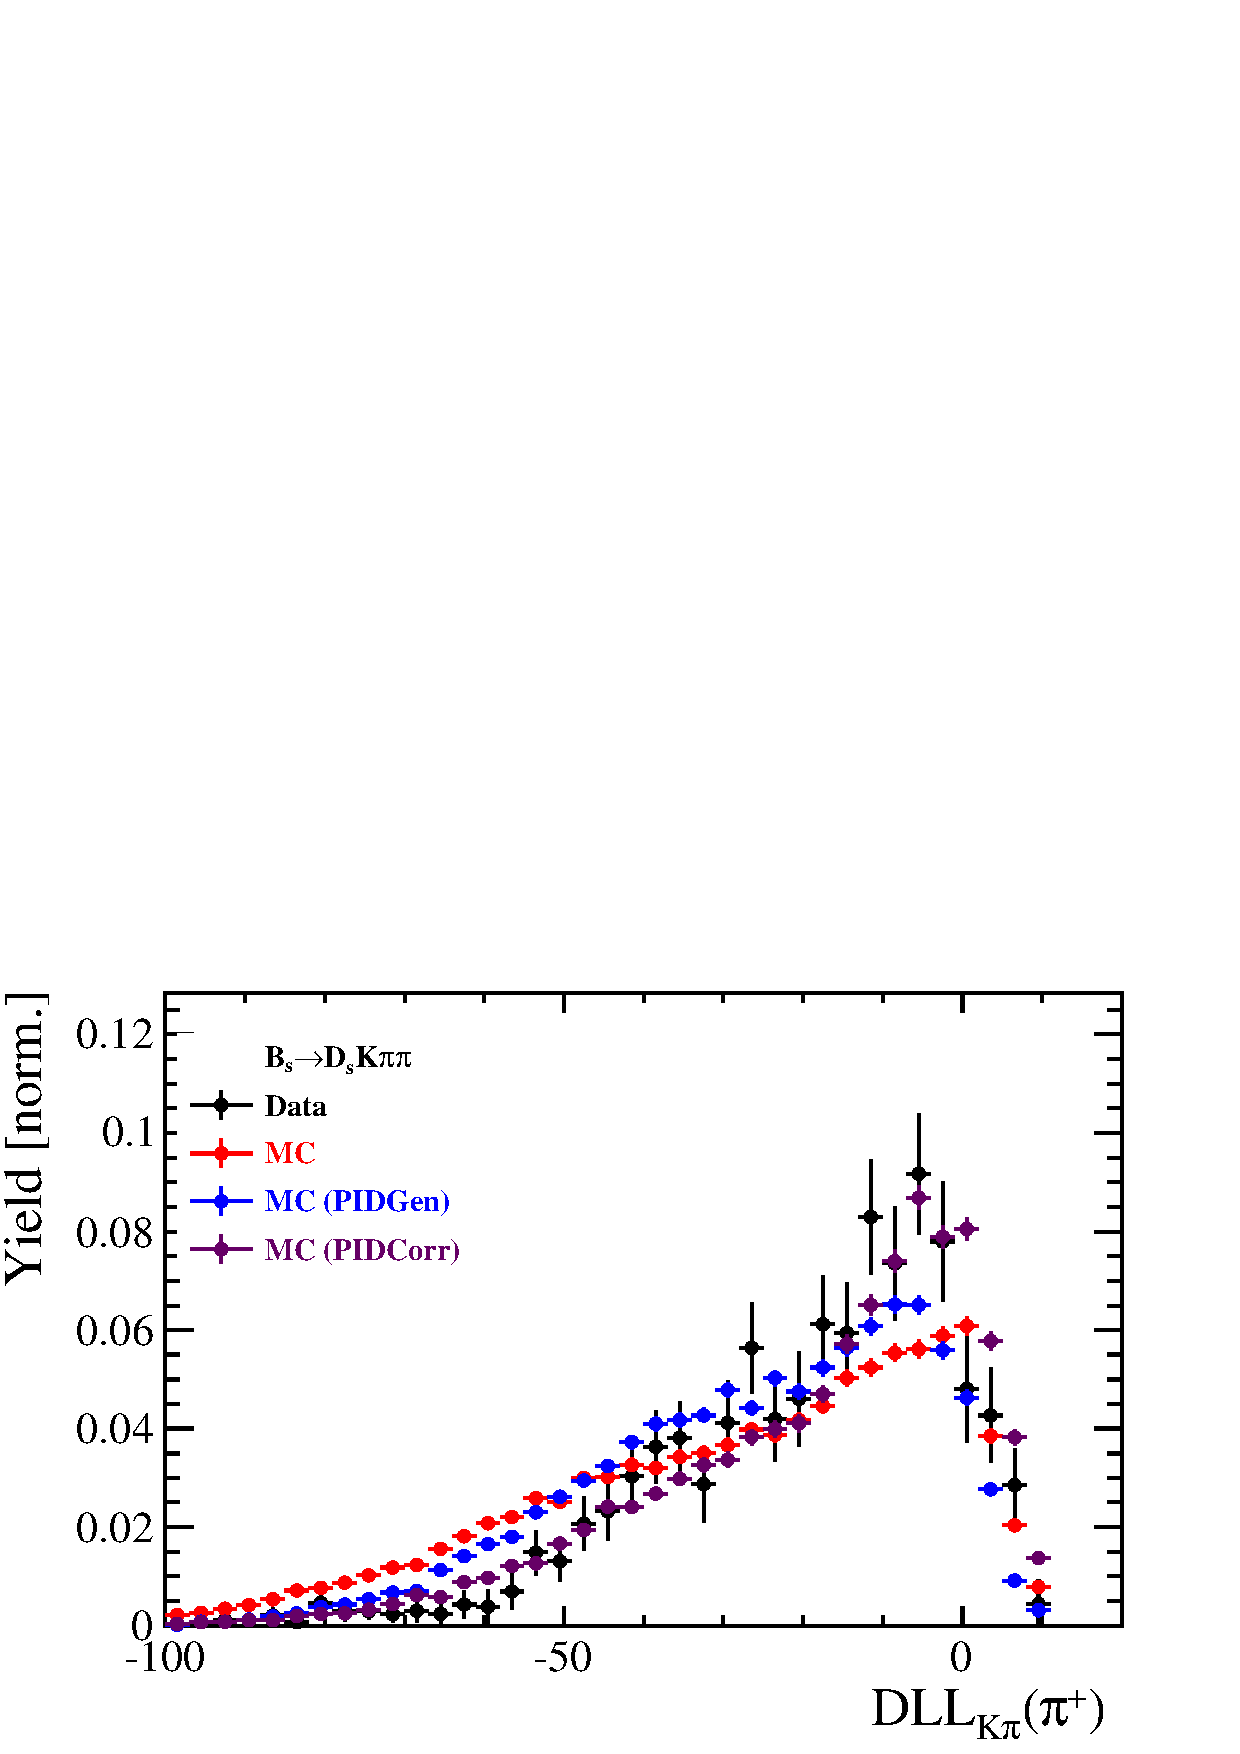
\includegraphics[height=!,width=0.32\textwidth]{figs/dataVsMC/signal_pid/PID_Ds2KKpi_1_pi_plus_PIDK.pdf}
%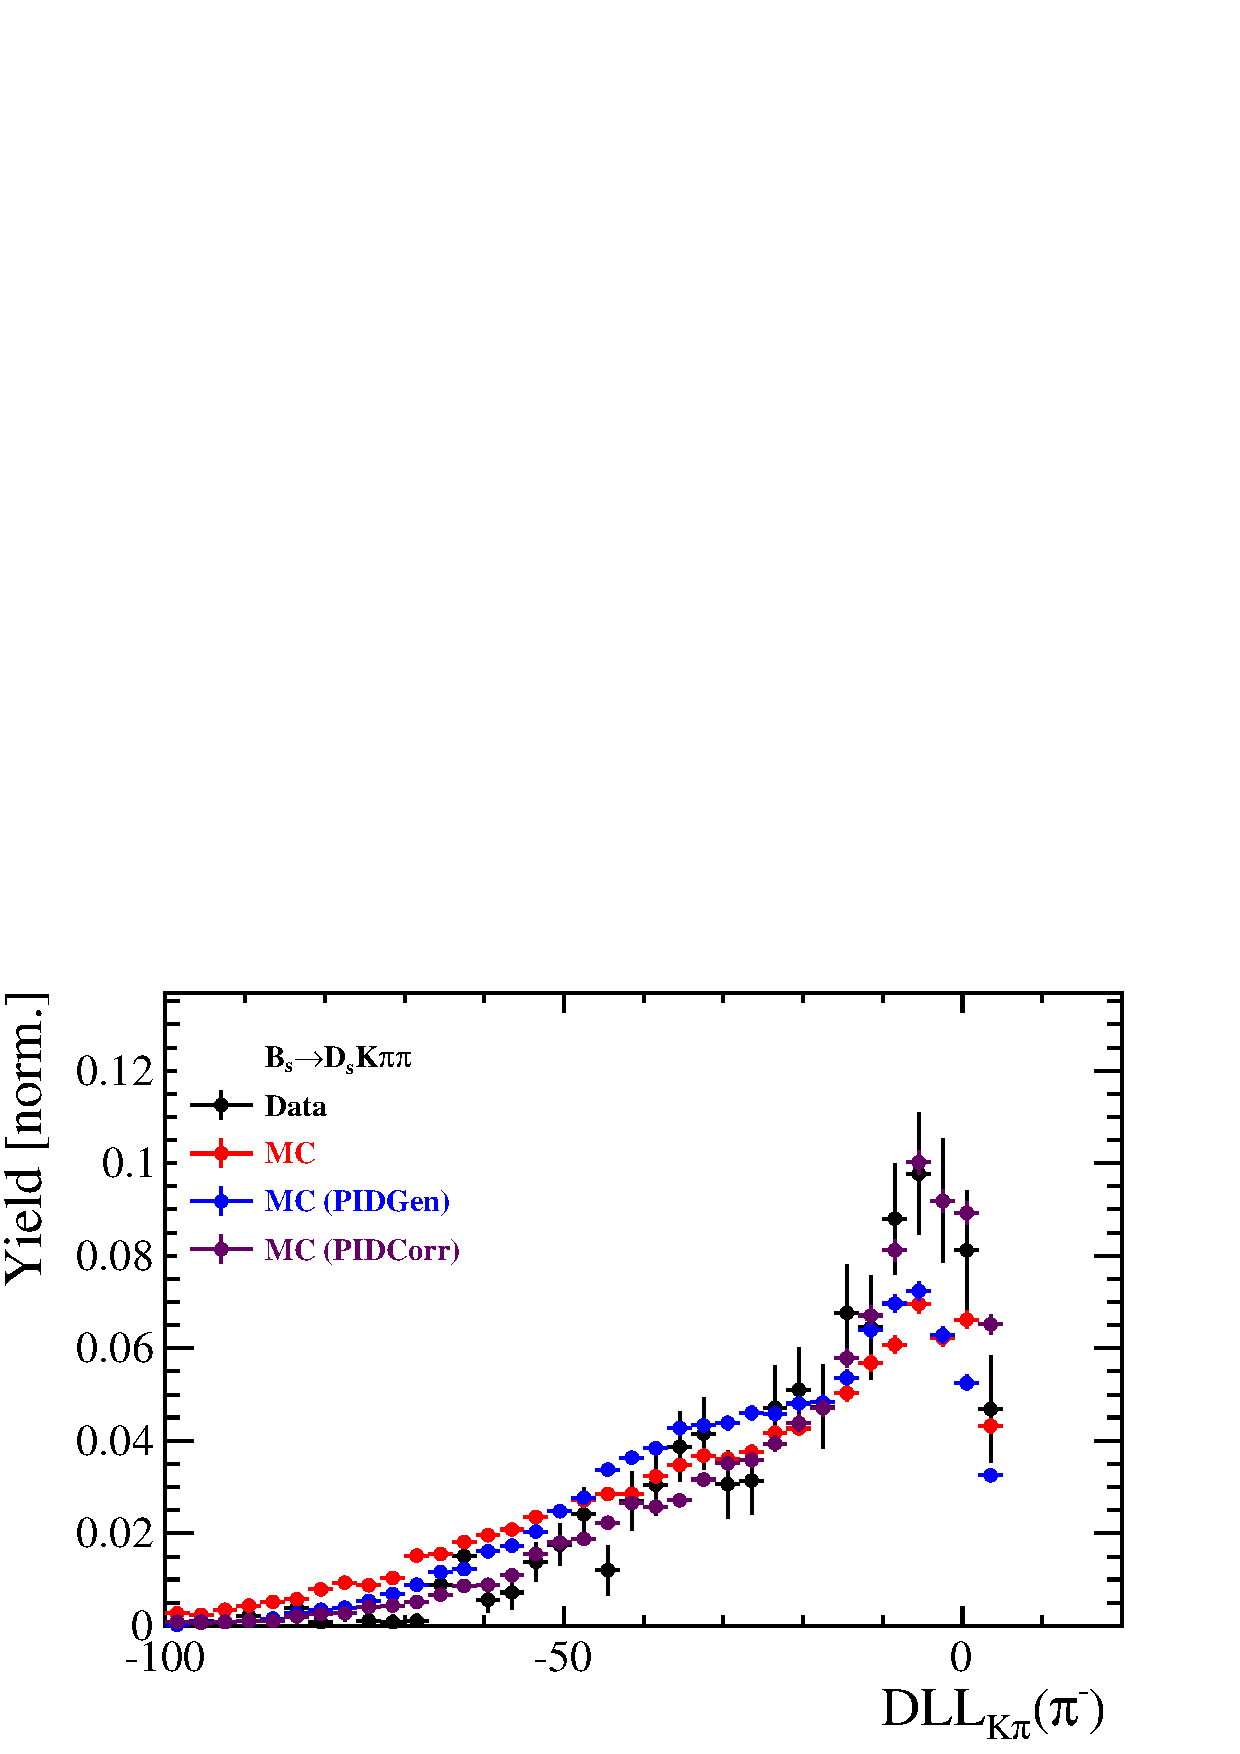
\includegraphics[height=!,width=0.32\textwidth]{figs/dataVsMC/signal_pid/PID_Ds2KKpi_1_pi_minus_PIDK.pdf}
%
%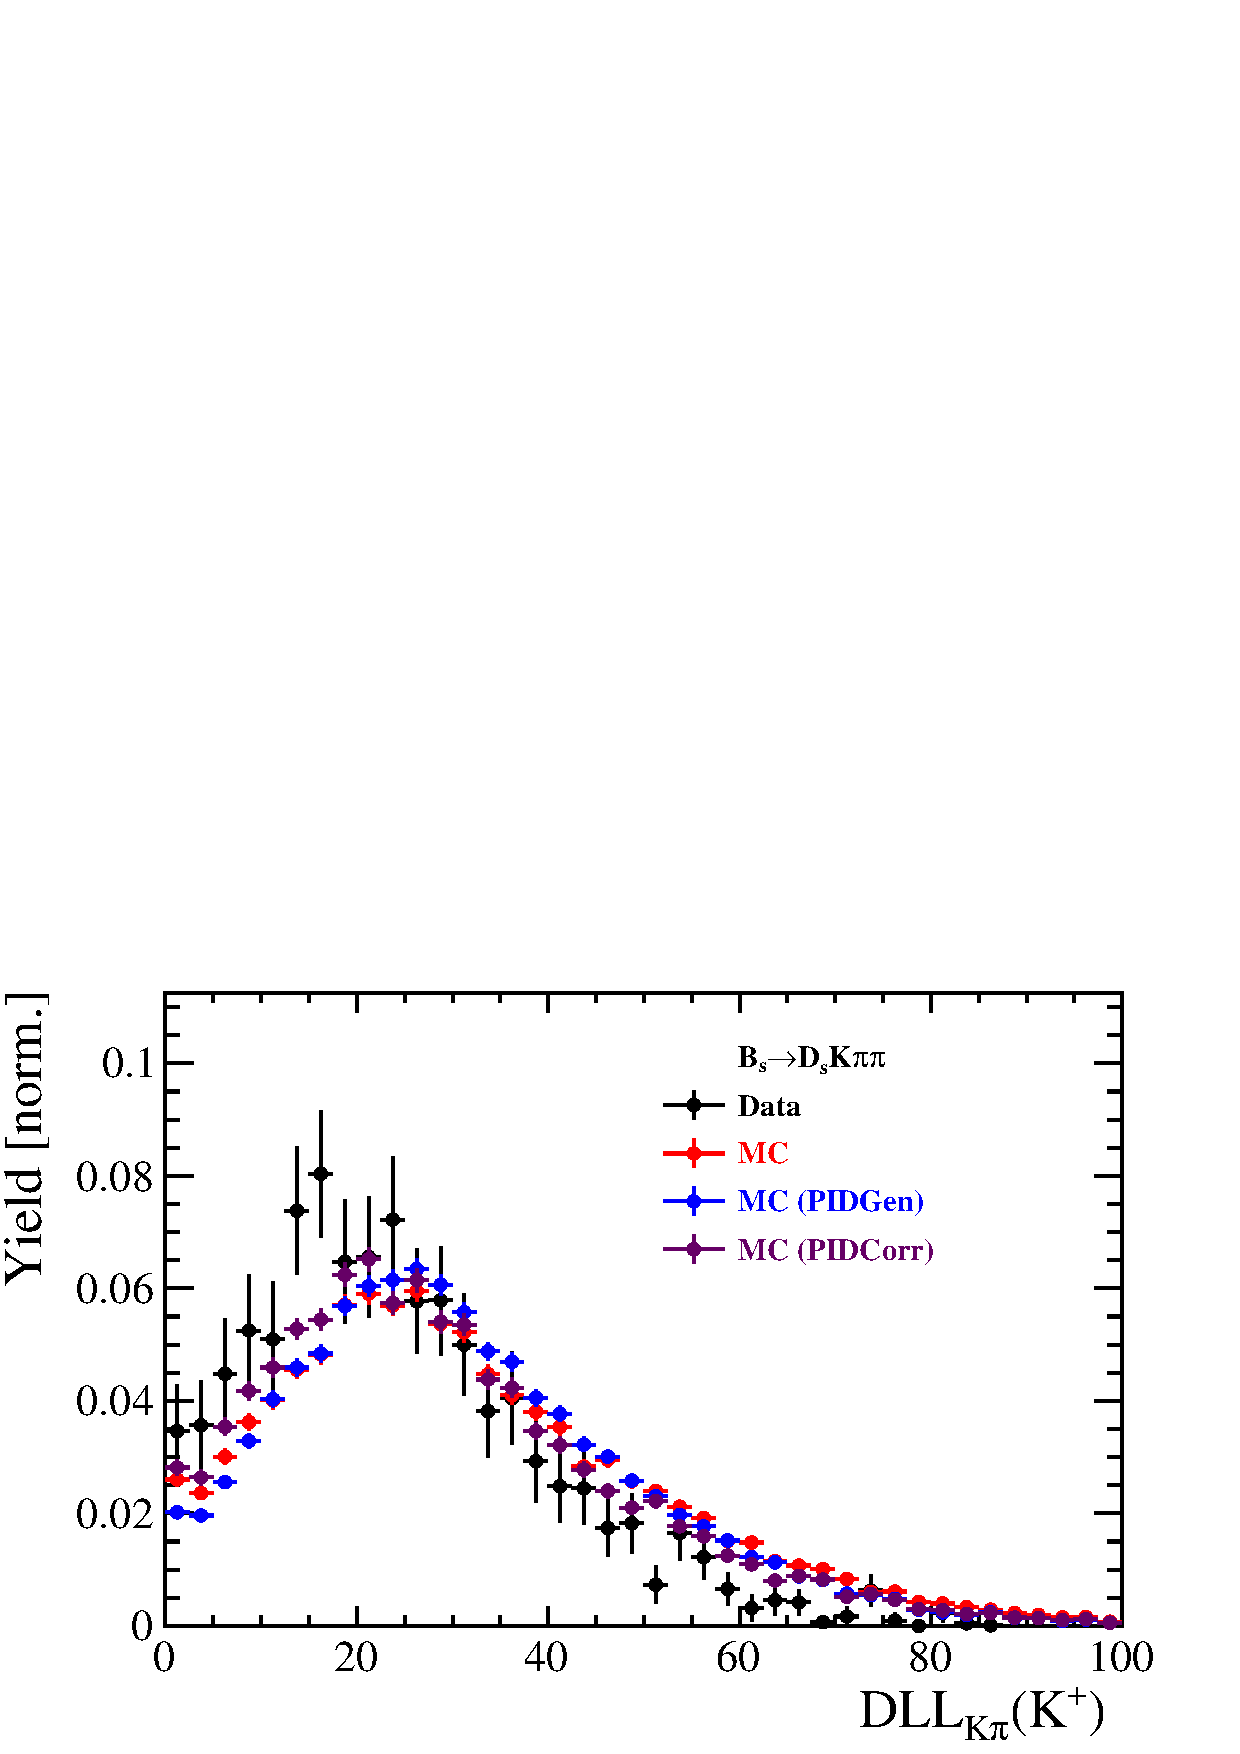
\includegraphics[height=!,width=0.32\textwidth]{figs/dataVsMC/signal_pid/PID_Ds2KKpi_1_K_plus_fromDs_PIDK.pdf}
%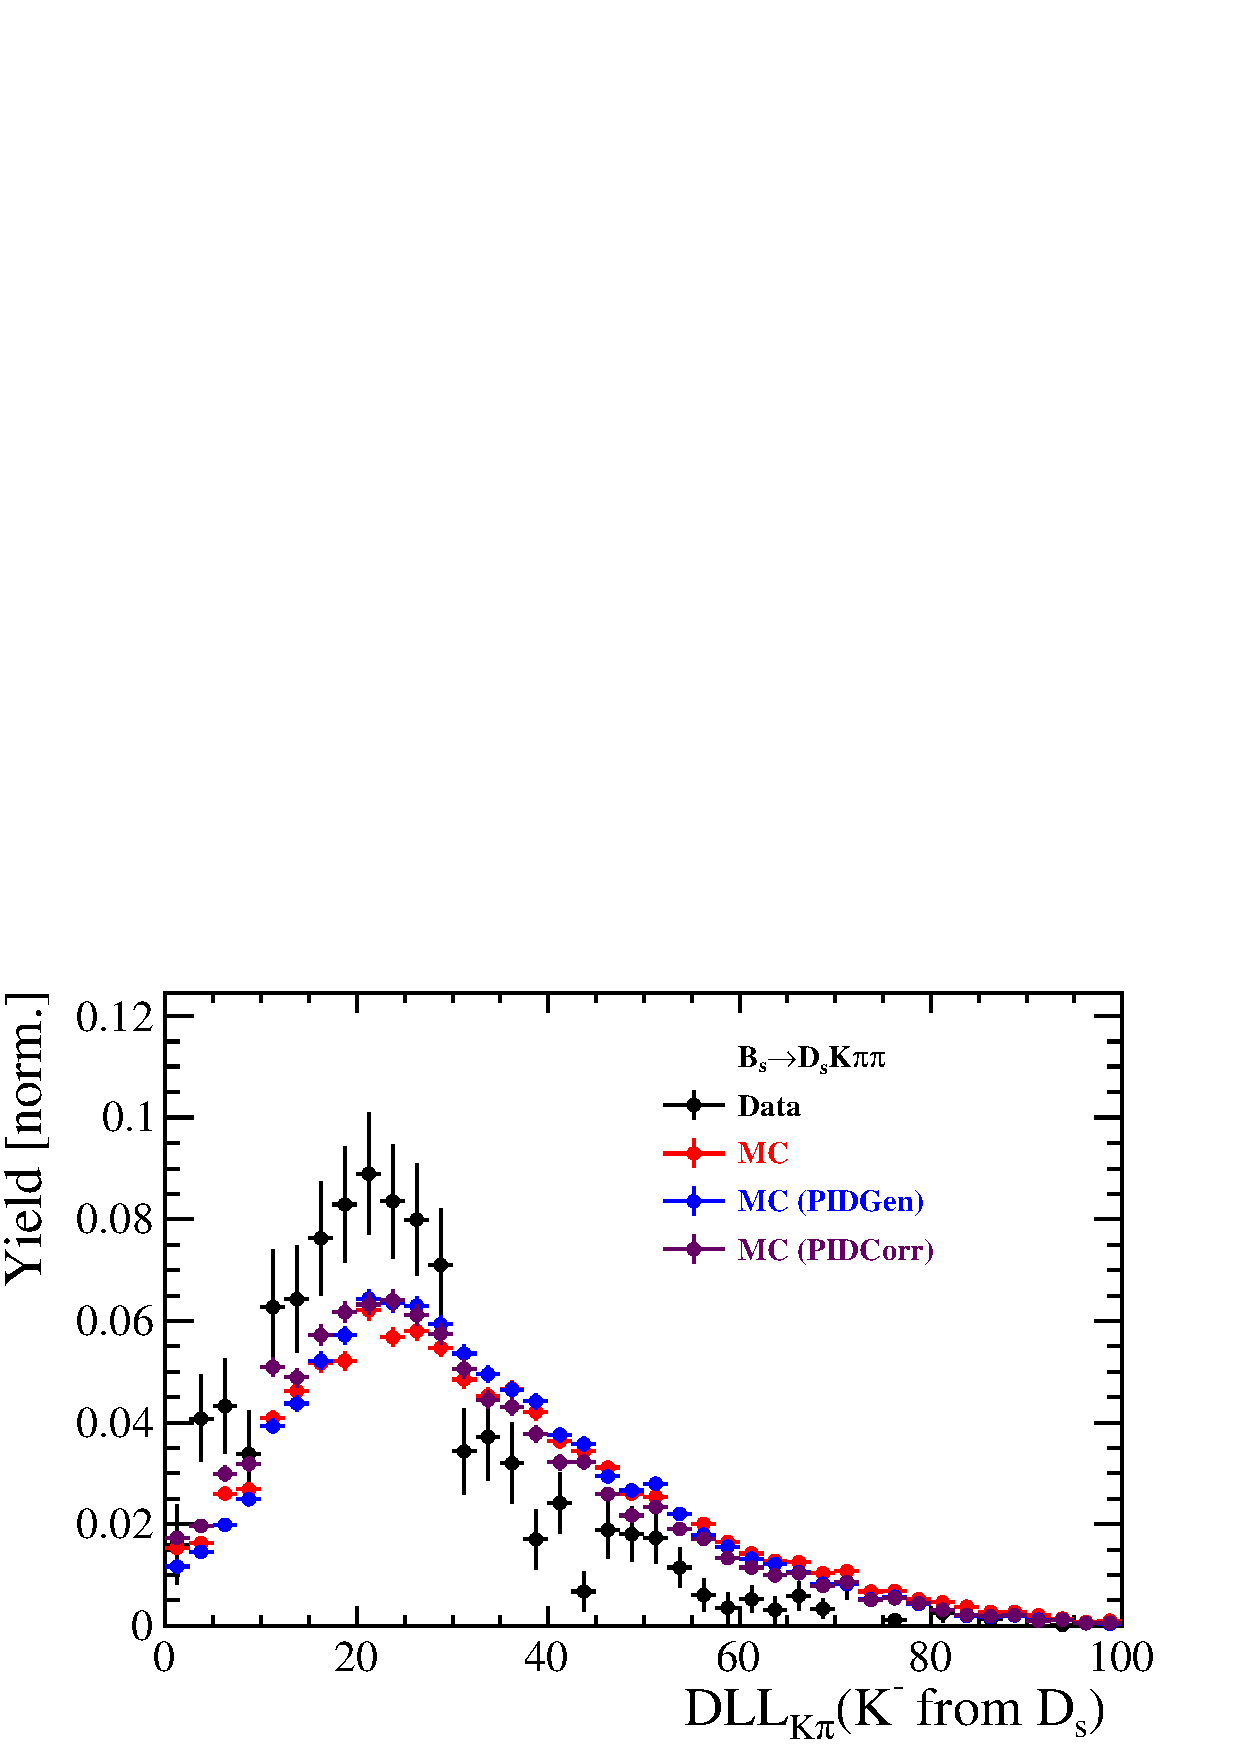
\includegraphics[height=!,width=0.32\textwidth]{figs/dataVsMC/signal_pid/PID_Ds2KKpi_1_K_minus_fromDs_PIDK.pdf}
%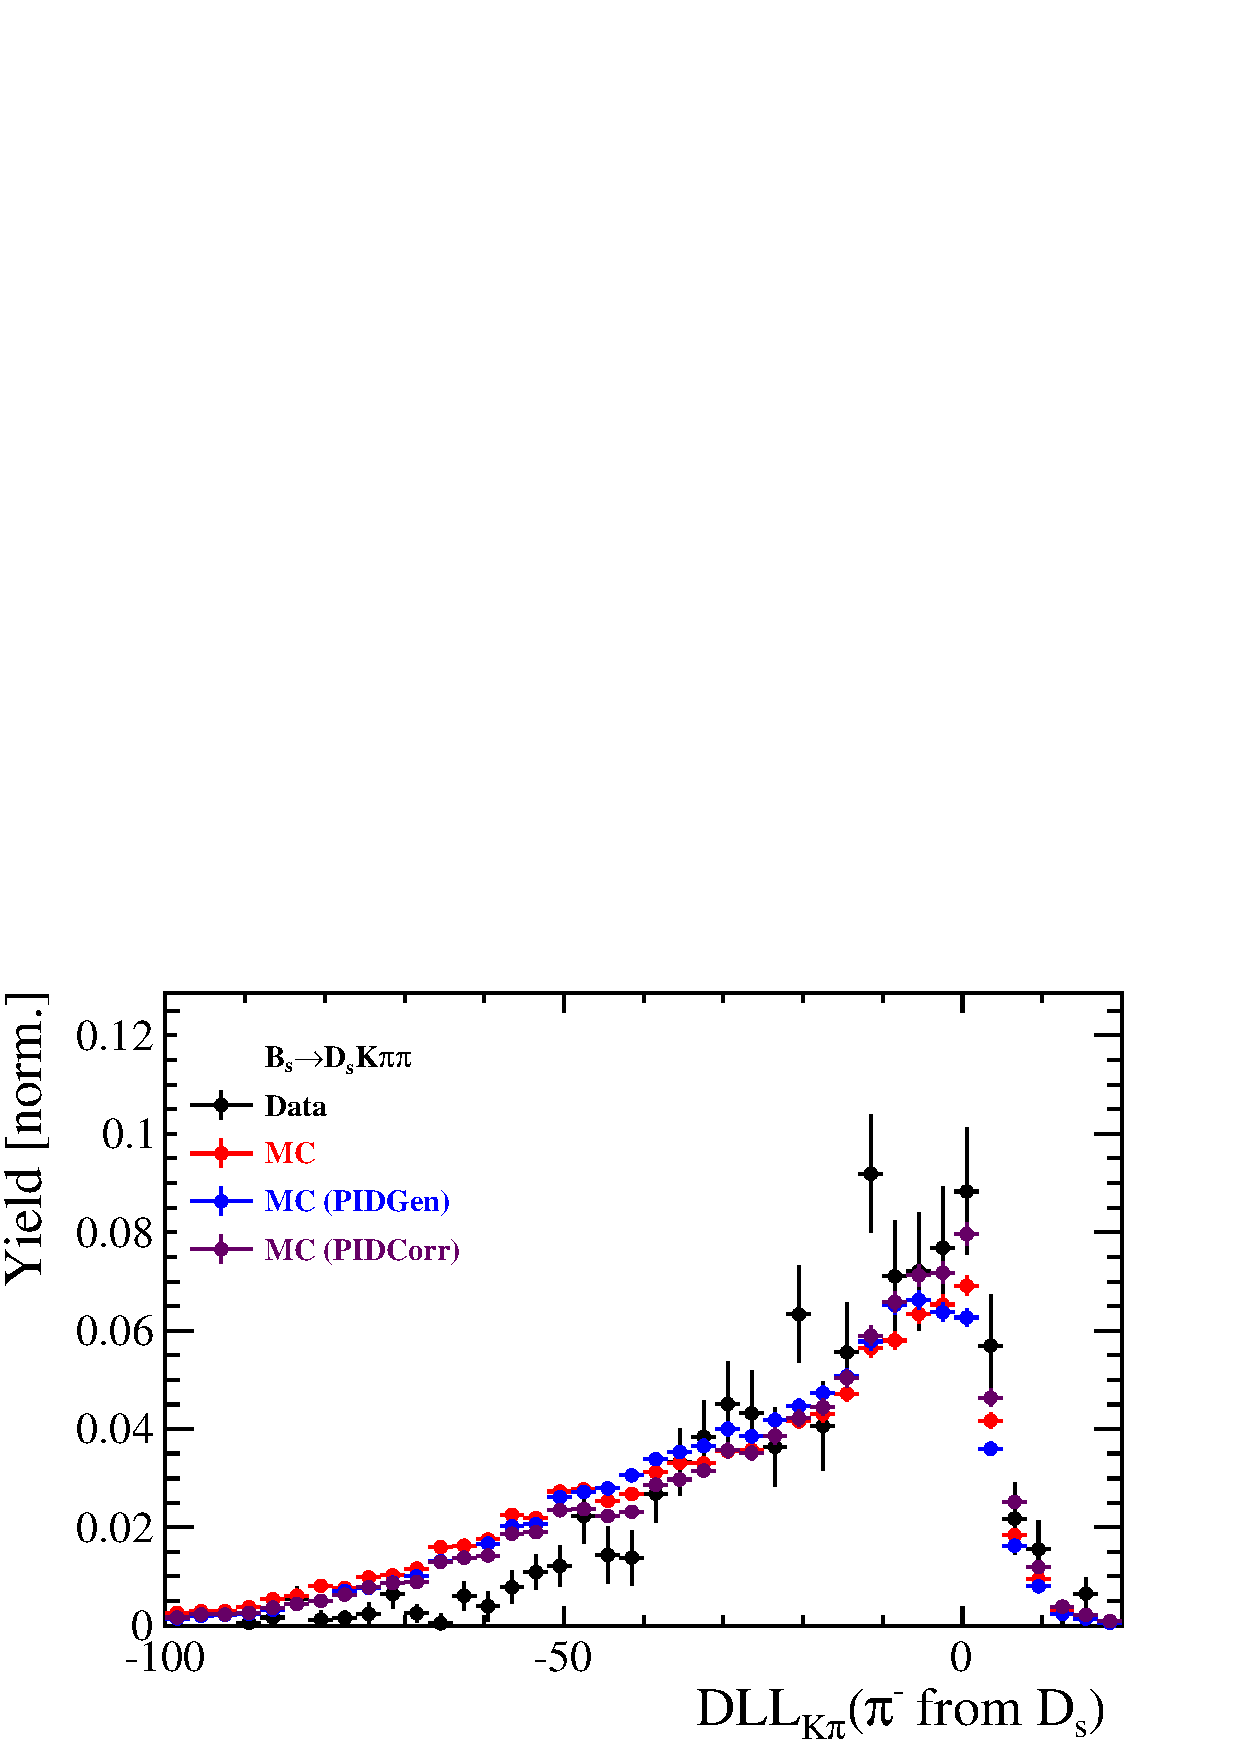
\includegraphics[height=!,width=0.32\textwidth]{figs/dataVsMC/signal_pid/PID_Ds2KKpi_1_pi_minus_fromDs_PIDK.pdf}
%\caption{}
%\label{fig:}
%\end{figure}
%
%\begin{figure}[h]
%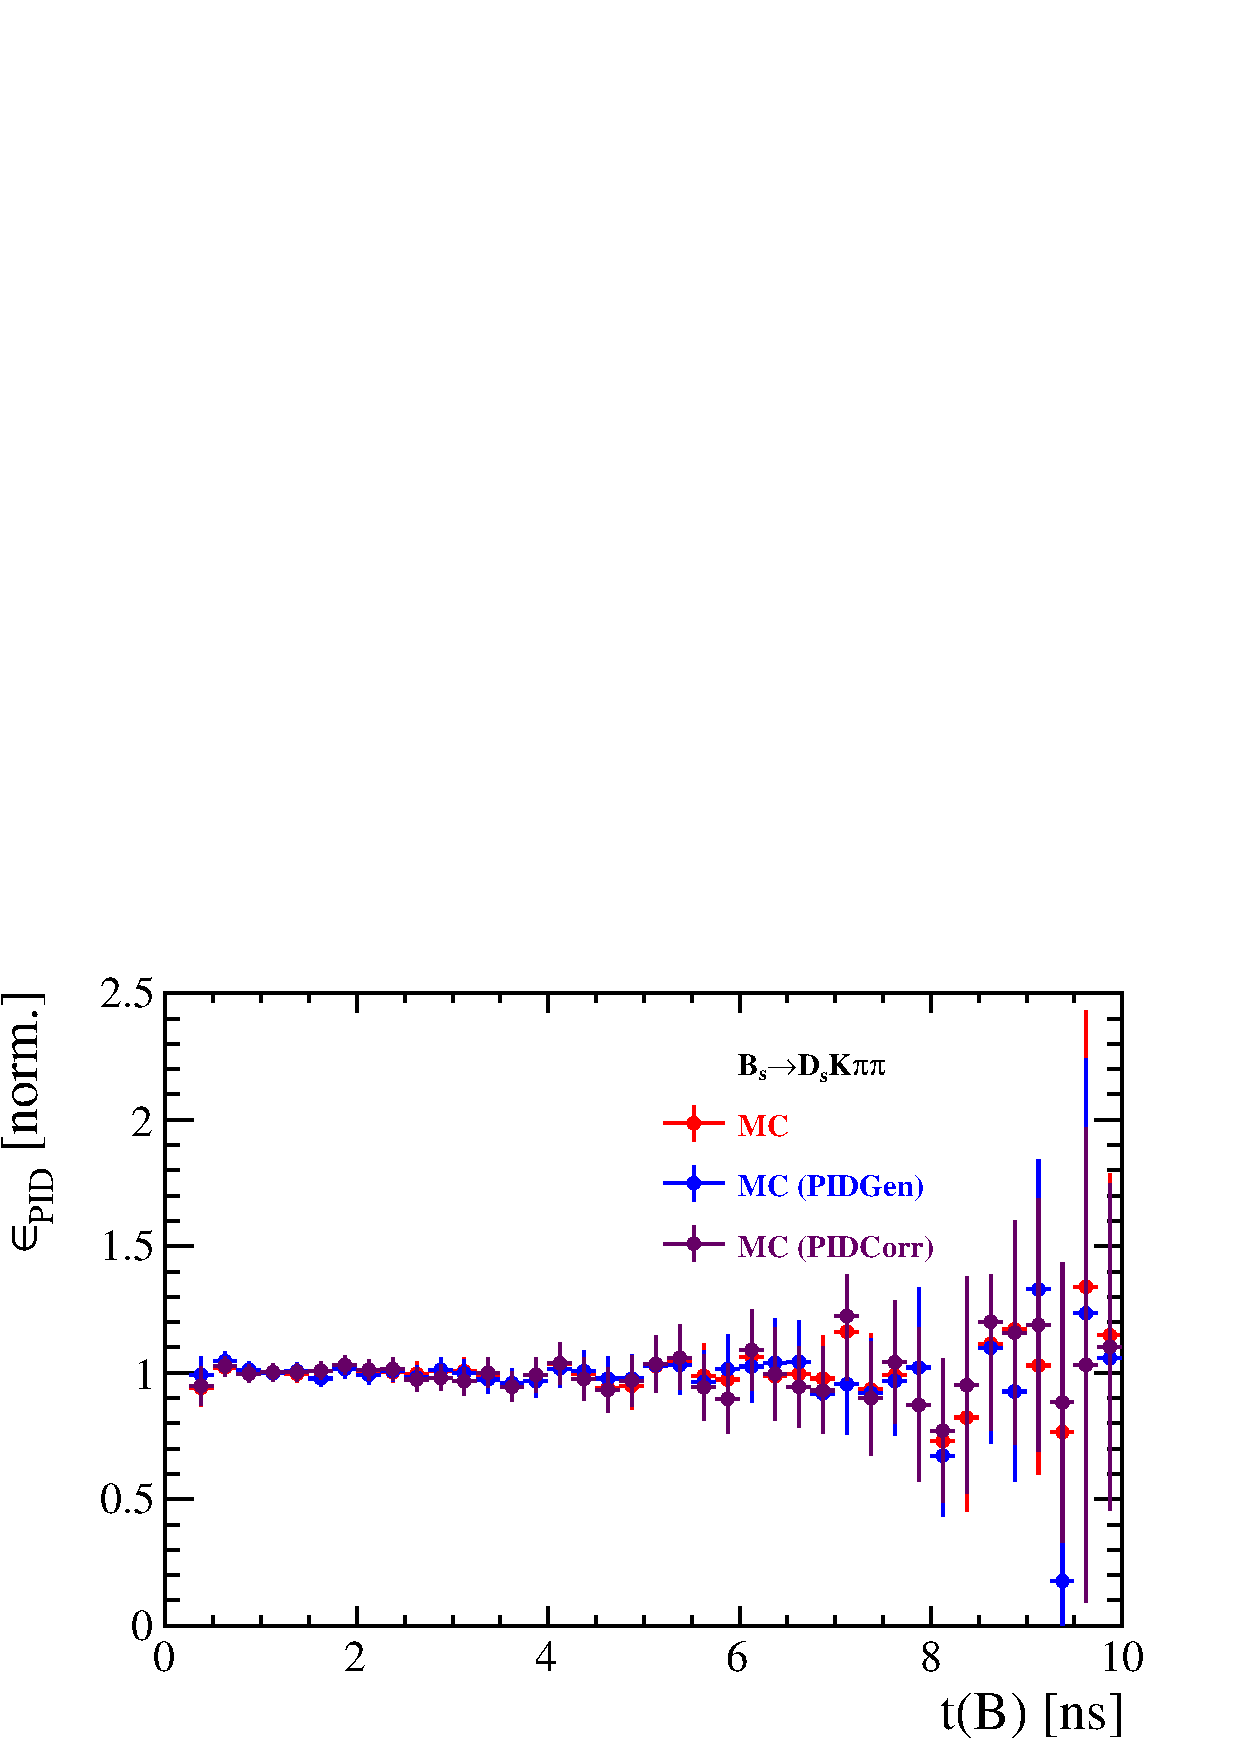
\includegraphics[height=!,width=0.32\textwidth]{figs/dataVsMC/signal_pid/eff_PID_Ds2KKpi_1_Bs_DTF_TAU.pdf}
%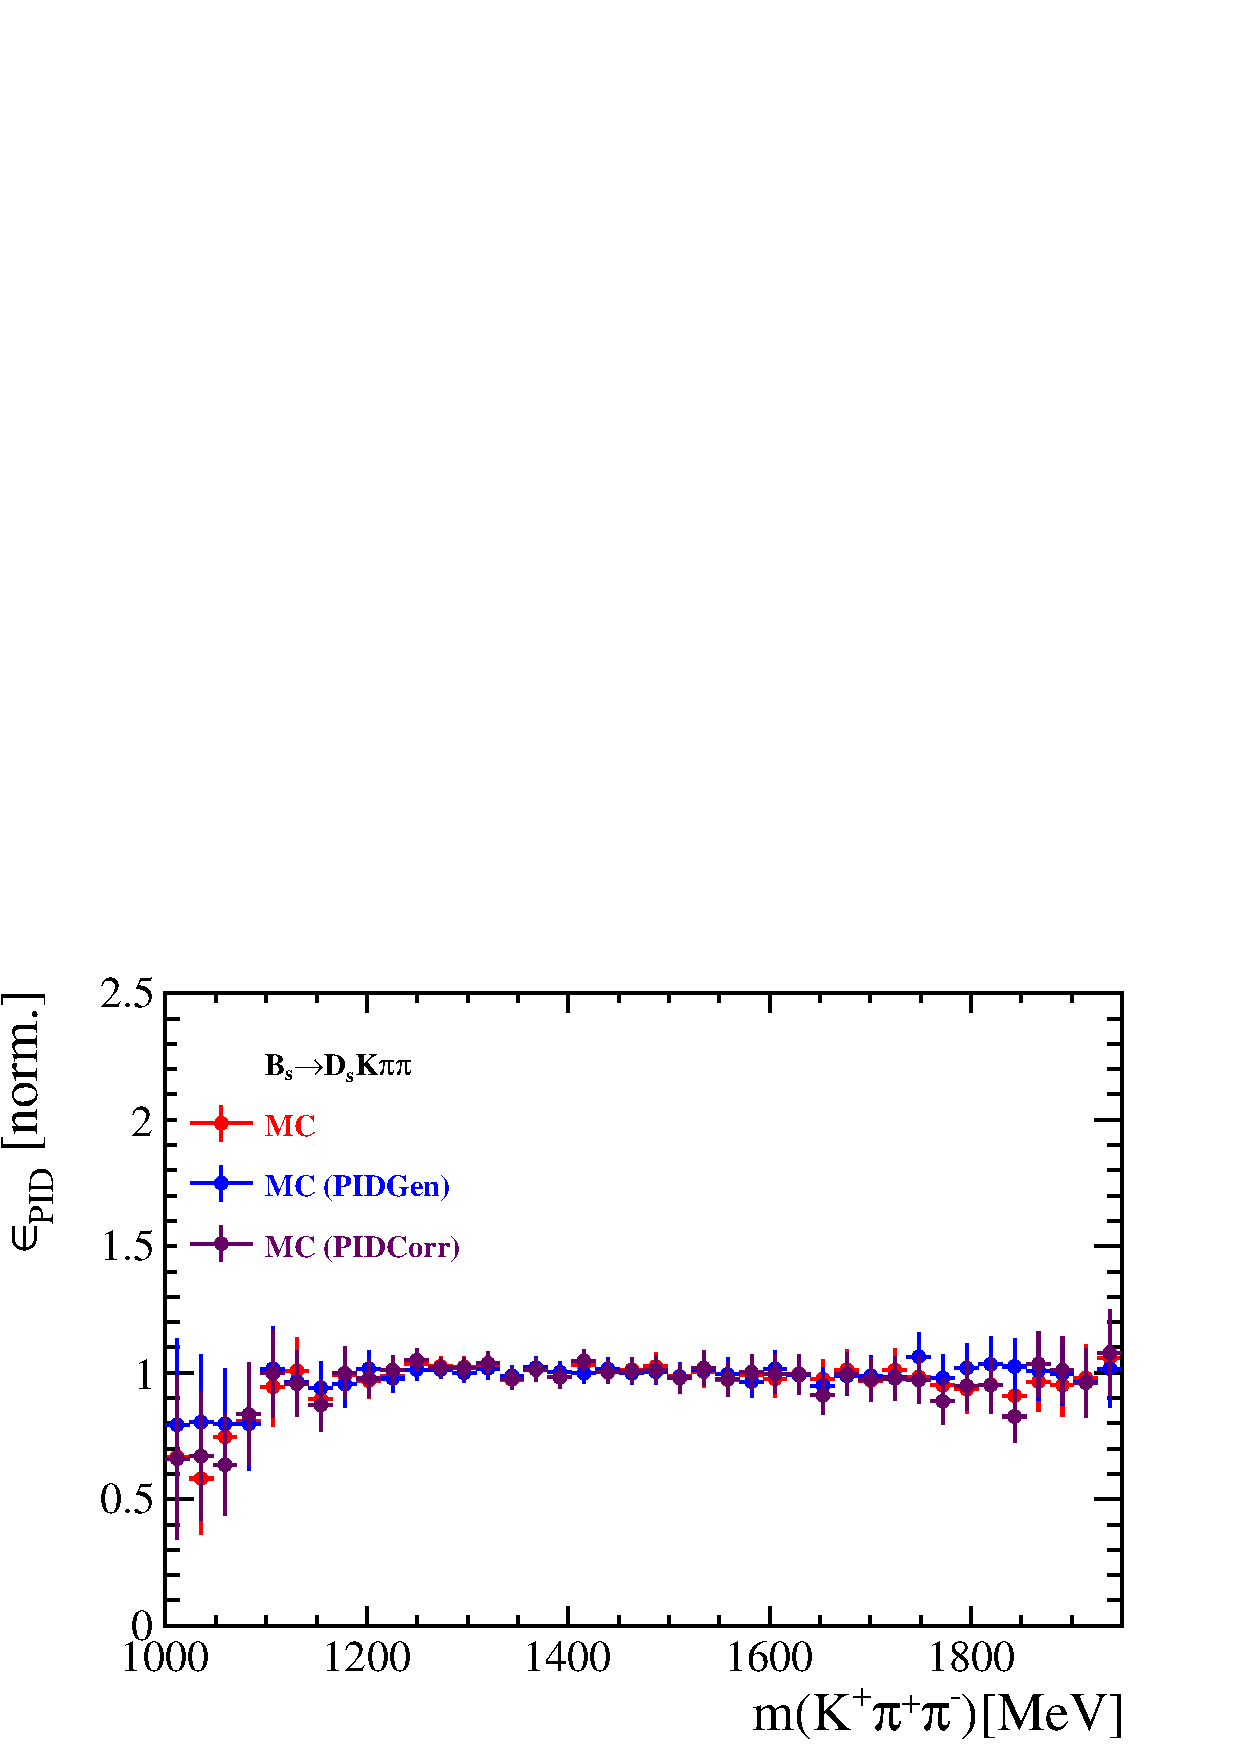
\includegraphics[height=!,width=0.32\textwidth]{figs/dataVsMC/signal_pid/eff_PID_Ds2KKpi_1_m_Kpipi.pdf}
%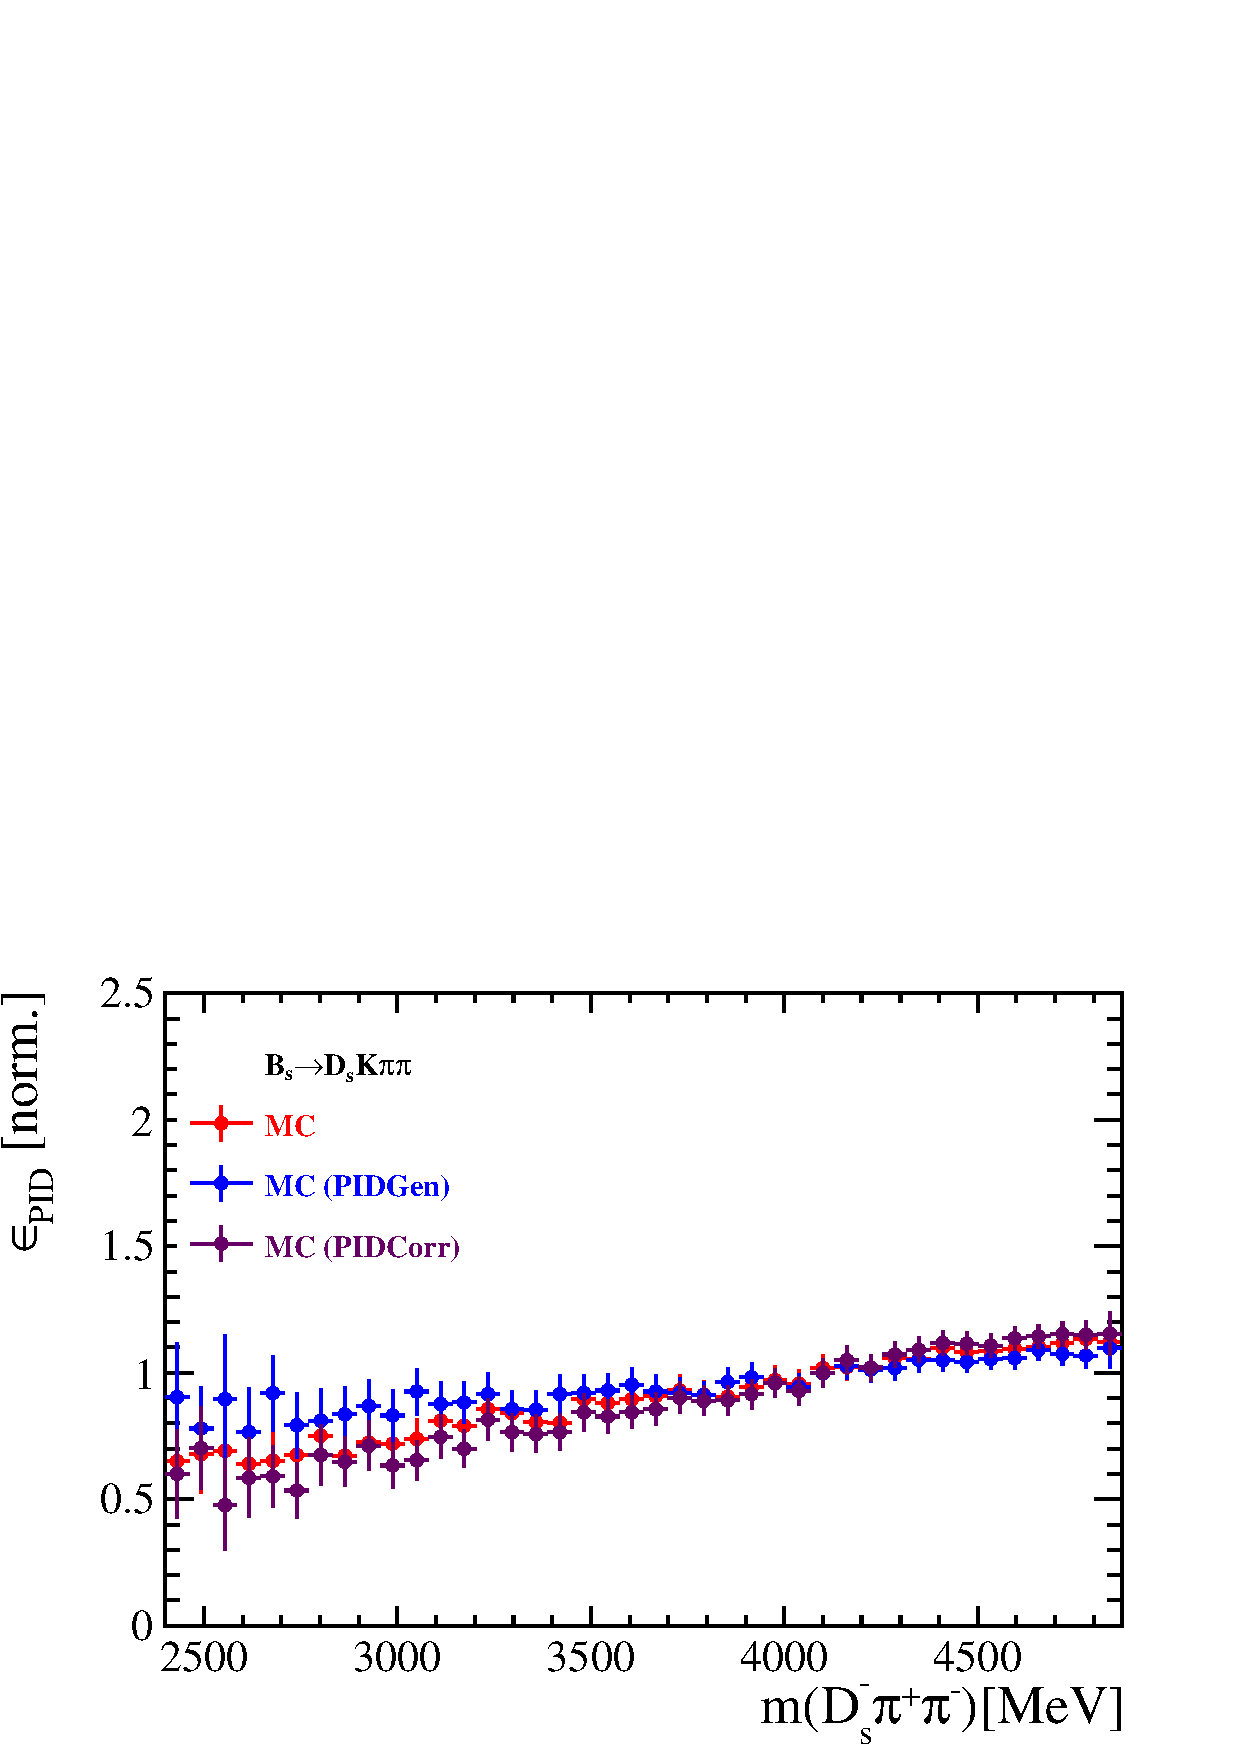
\includegraphics[height=!,width=0.32\textwidth]{figs/dataVsMC/signal_pid/eff_PID_Ds2KKpi_1_m_Dspipi.pdf}
%
%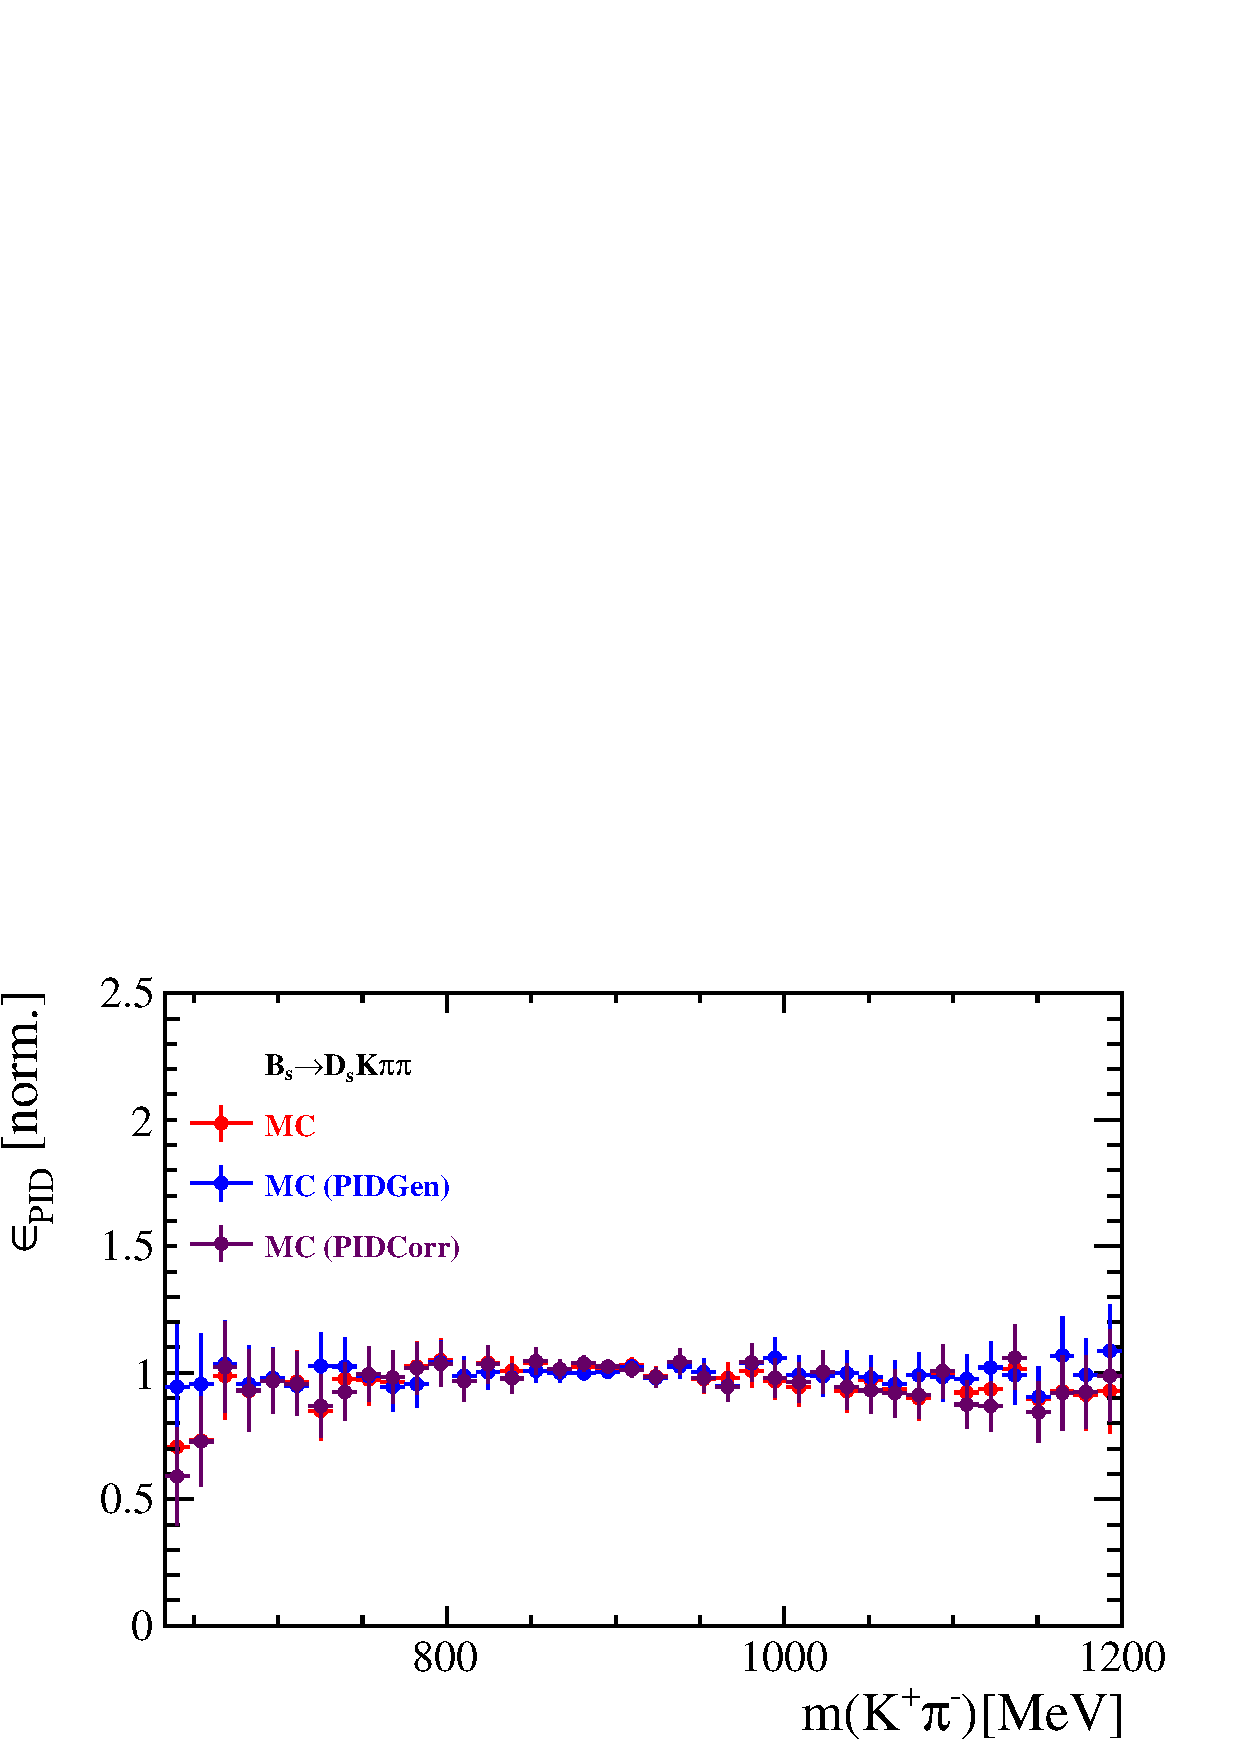
\includegraphics[height=!,width=0.32\textwidth]{figs/dataVsMC/signal_pid/eff_PID_Ds2KKpi_1_m_Kpi.pdf}
%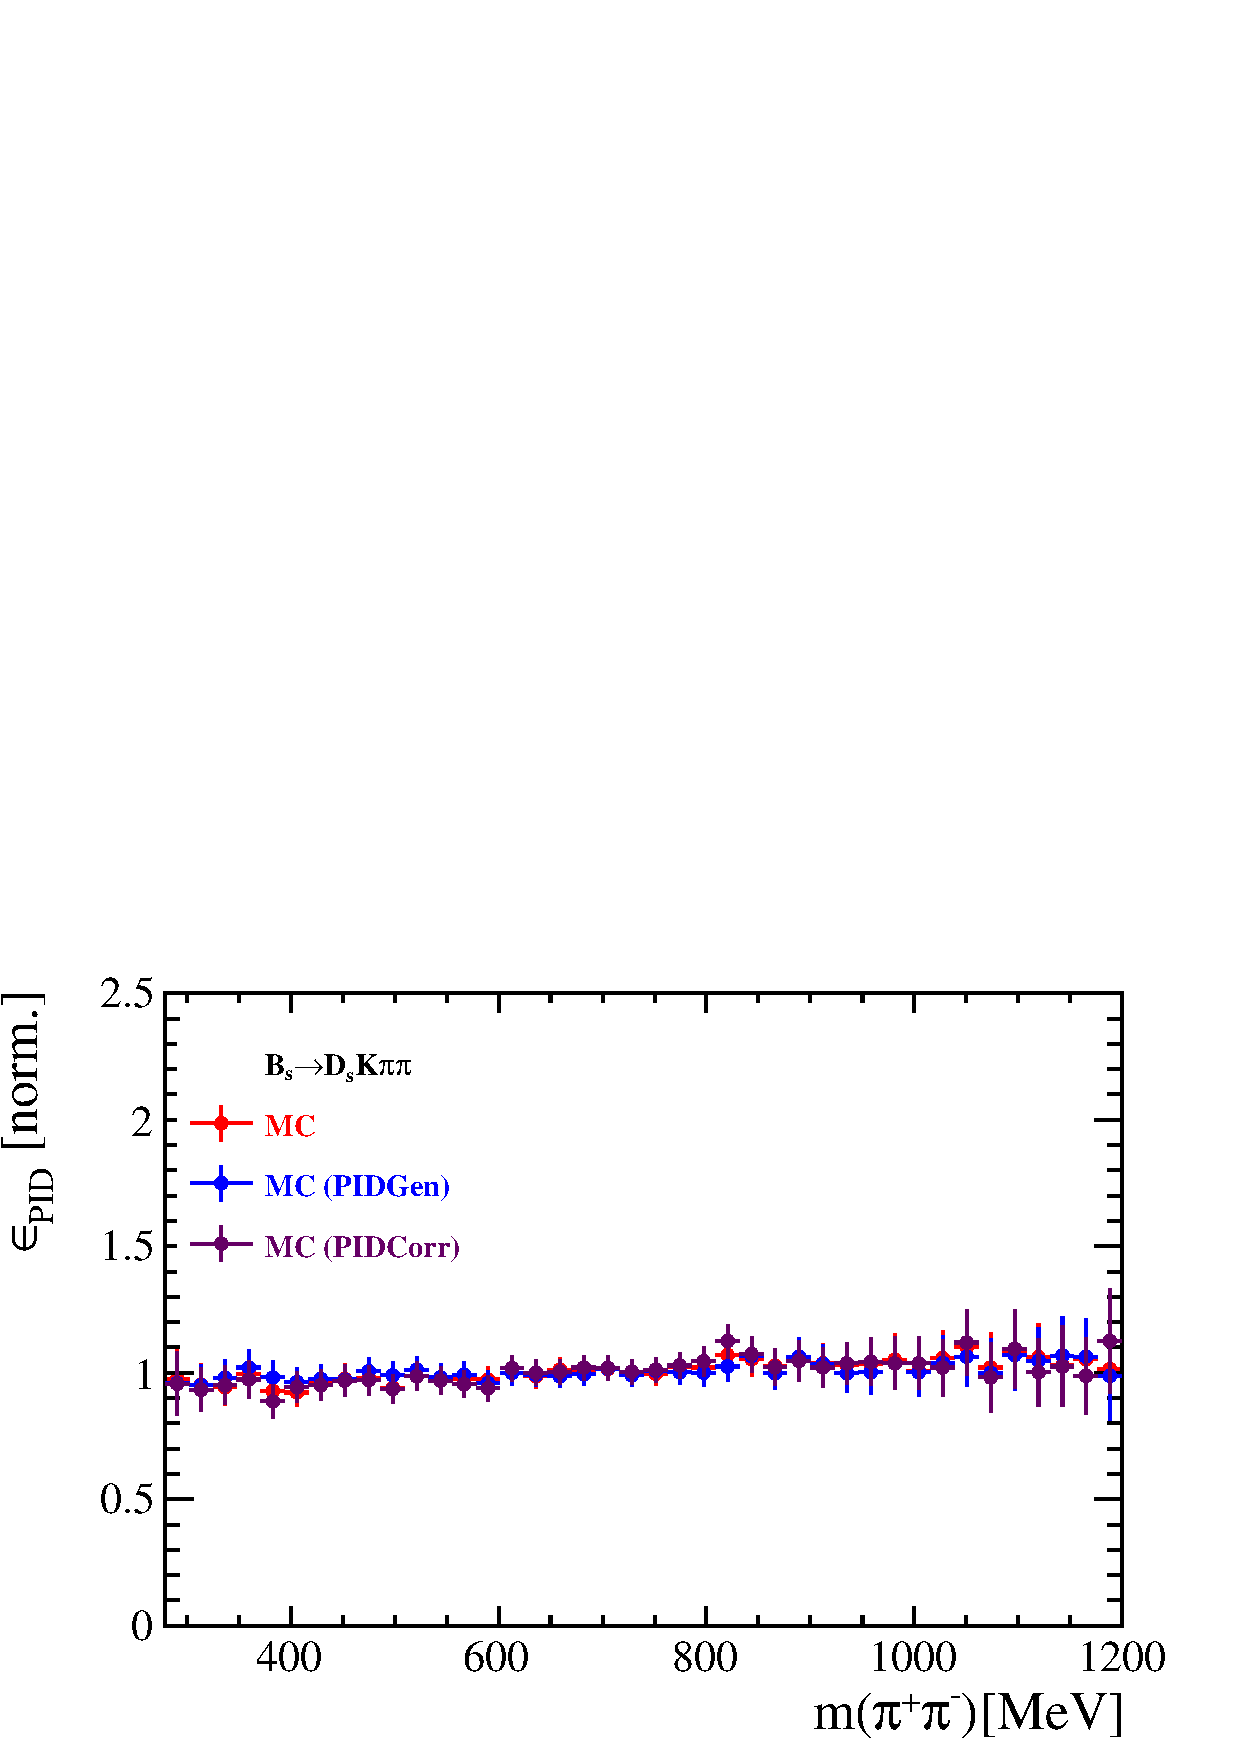
\includegraphics[height=!,width=0.32\textwidth]{figs/dataVsMC/signal_pid/eff_PID_Ds2KKpi_1_m_pipi.pdf}
%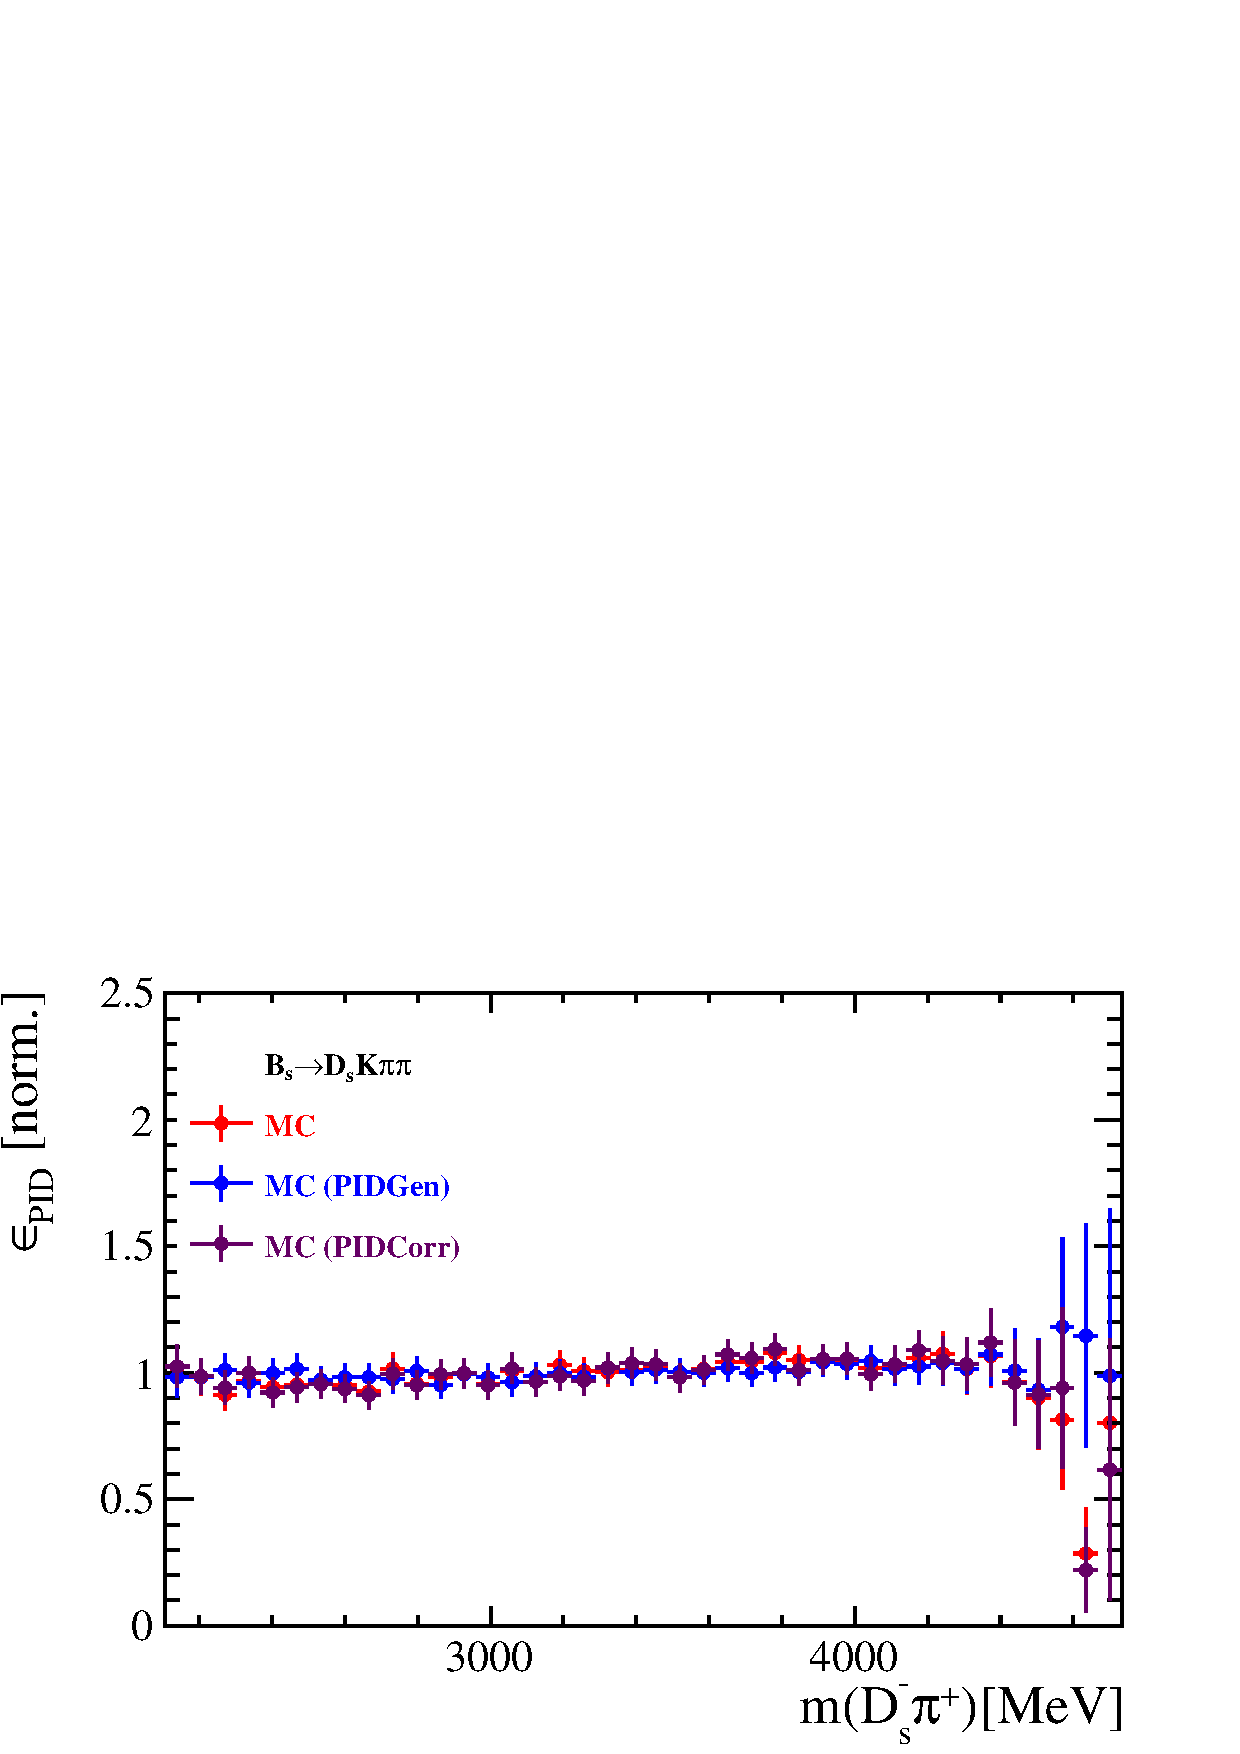
\includegraphics[height=!,width=0.32\textwidth]{figs/dataVsMC/signal_pid/eff_PID_Ds2KKpi_1_m_Dspi.pdf}
%\caption{}
%\label{fig:}
%\end{figure}
%
%
%\clearpage
%\subsubsection{BDT efficiencies}
%
%\begin{figure}[h]
%\includegraphics[height=!,width=0.32\textwidth]{figs/dataVsMC/signal_bdt/eff_Ds2KKpi_1_Bs_DTF_TAU.pdf}
%\includegraphics[height=!,width=0.32\textwidth]{figs/dataVsMC/signal_bdt/eff_Ds2KKpi_1_m_Kpipi.pdf}
%\includegraphics[height=!,width=0.32\textwidth]{figs/dataVsMC/signal_bdt/eff_Ds2KKpi_1_m_Dspipi.pdf}
%
%\includegraphics[height=!,width=0.32\textwidth]{figs/dataVsMC/signal_bdt/eff_Ds2KKpi_1_m_Kpi.pdf}
%\includegraphics[height=!,width=0.32\textwidth]{figs/dataVsMC/signal_bdt/eff_Ds2KKpi_1_m_pipi.pdf}
%\includegraphics[height=!,width=0.32\textwidth]{figs/dataVsMC/signal_bdt/eff_Ds2KKpi_1_m_Dspi.pdf}
%\caption{}
%\label{fig:}
%\end{figure}
%
%
%\begin{figure}[h]
%\includegraphics[height=!,width=0.32\textwidth]{figs/dataVsMC/signal_bdt_scan/eff_Ds2KKpi_1_Bs_DTF_TAU.pdf}
%\includegraphics[height=!,width=0.32\textwidth]{figs/dataVsMC/signal_bdt_scan/eff_Ds2KKpi_1_m_Kpipi.pdf}
%\includegraphics[height=!,width=0.32\textwidth]{figs/dataVsMC/signal_bdt_scan/eff_Ds2KKpi_1_m_Dspipi.pdf}
%
%\includegraphics[height=!,width=0.32\textwidth]{figs/dataVsMC/signal_bdt_scan/eff_Ds2KKpi_1_m_Kpi.pdf}
%\includegraphics[height=!,width=0.32\textwidth]{figs/dataVsMC/signal_bdt_scan/eff_Ds2KKpi_1_m_pipi.pdf}
%\includegraphics[height=!,width=0.32\textwidth]{figs/dataVsMC/signal_bdt_scan/eff_Ds2KKpi_1_m_Dspi.pdf}
%\caption{}
%\label{fig:}
%\end{figure}
%
%
%\clearpage
%\subsubsection{Tracking efficiencies}

\clearpage

\subsection{Decay-time acceptance}
\label{sec:timeAcceptance}
The decay-time distribution of the $\Bs$ mesons is sculpted due to the geometry of the LHCb detector and the applied selection cuts, which are described in Section \ref{sec:Selection}.
In particular, any requirement on the flight distance, the impact parameter or the direction angle (DIRA) of the $\Bs$ mesons, as well as the direct cut on the proper-time, will lead to a decay-time dependent efficiency $\epsilon(t)$. 
%This efficiency will distort the theoretically expected, time-dependent decay rate
%\begin{equation}
%\frac{\Gamma(t)^{observed}}{dt} = \frac{\Gamma(t)^{theory}}{dt} \cdot \epsilon(t),
%\label{eq:DecRateAcc}
%\end{equation} 
%and has to be modelled correctly, in order to describe the observed decay rate. 

We use a combination of control channels to derive the acceptance function $\epsilon(t)$, because for $\Bs\to\Ds\kaon\pion\pion$ decays the decay-time acceptance is strongly correlated with the \CP-observables which we aim to measure. Therefore, extracting the \CP-observables and the acceptance shape at the same time is not possible. 
A fit to the decay-time distribution of $\Bs\to\Ds\pion\pion\pion$ candidates is performed and the obtained acceptance shape is corrected for the small difference 
observed between the $\Bs\to\Ds\kaon\pion\pion$ and $\Bs\to\Ds\pion\pion\pion$ MC samples. 
In addition, we include the control channel $\Bd\to\Ds\kaon\pion\pion$ to increase the statistical precision.
A simultaneous fit to the four datasets ($\Bs\to\Ds\pion\pion\pion$ data, $\Bd\to\Ds\kaon\pion\pion$ data, $\Bs\to\Ds\kaon\pion\pion$ MC and $\Bs\to\Ds\pion\pion\pion$ MC)
is performed to allow for a straightforward propagation of uncertainties.
In each case, a PDF of the following form 
\begin{equation}
\mathcal{P}(t,\delta t) = \left[ e^{-\Gamma \, t}\cdot \text{cosh}\left(\frac{\Delta\Gamma \, t^\prime}{2}\right) \otimes \mathcal{R}(t - t^{'}, \delta t)\right] \cdot \epsilon(t),
\label{eq:AccPDF}
\end{equation}
is used to describe the decay-time distribution. 
For real data, the values for $\Gamma_{s,d}$ and $\Delta\Gamma_{s,d}$ are fixed to the latest HFLAV results \cite{HFAG},
while for simulated data, the generated values are used.
A  single Gaussian resolution function $\mathcal{R}(t - t^{'}, \delta t)$ is used where the decay-time error estimate is scaled with the respective calibration functions determined in
Sec.~\ref{sec:Resolution}.
Each decay-time acceptance $\epsilon(t)$ is modeled
using cubic splines, allowing for the analytical computation of the decay-time integrals appearing in the PDF \cite{Karbach:2014qba}.
The splines are parametrized by so-called knots ($t_0,t_1,\dots,t_N$) which determine their boundaries. 
Two knots are located by default at the lower and upper edge of the interval allowed for the decay time, the remaining ones are chosen 
such that there is an approximately equal amount of data in-between two consecutive knots.
In the basis of cubic b-splines, $b_i(t)$, the acceptance is then constructed as:
\begin{equation}   
	\epsilon(t) = \sum_{i=0}^N v_i \, b_i(t)   
	\label{eq:Spline}
\end{equation}
where the spline coefficients $v_i$ are determined from the fit.
% using the sum of cubic polynomials $v_{i}(t)$, so called Splines \cite{Karbach:2014qba}. 
%Knots can be set across the fitted distribution to account for local changes in the acceptance shape.
%Using more knots is equivalent to using more base splines which are defined on a smaller sub-range. 
%In total, $n+2$ base splines $v_{i}(t)$ are needed to describe an acceptance shape which is parametrized using $n$ knots.
%For fits shown in the following, the knots have been placed at $t = [0.5, 1.0, 1.5, 2.0, 3.0, 9.5] ps$. 
%To accommodate these 6 knot positions, 8 basic splines $v_{i}$, $i = [1,...,8]$ are used.
%Since a rapid change of the decay time acceptance at low decay times due to the turn-on effect generated by the lifetime and other selection cuts is expected, more knots are placed in that regime.
%At higher decay times we expect linear behavior, with a possible small effect due to the VELO reconstruction. Therefore fewer knots are used. 
We fix coefficient $v_{N-1}$ to unity in order to normalize the overall acceptance function. 
To stabilize the upper decay-time acceptance, $v_{N}$ is fixed by a linear extrapolation from the two previous coefficients:
\begin{equation}   
v_{N} = v_{N-1} + \frac{v_{N-2} - v_{N-1}}{t_{N-2} - t_{N-1}} \cdot (t_{N} - t_{N-1}).
\label{eq:SplineExtra}
\end{equation}
It was found that at least $N=6$ knots are necessary for a sufficient fit quality.

\clearpage
Three distinct splines are used in the following combinations to describe the acceptances for the
four datasets:
\begin{itemize}
	\item $\Bs \to D_sK\pi\pi$ MC:   $\epsilon^{MC}_{D_sK\pi\pi}(t)$ 
	\item $\Bs \to D_s\pi\pi\pi$ MC:   $\epsilon^{MC}_{D_s\pi\pi\pi}(t) = R(t) \cdot \epsilon^{MC}_{D_sK\pi\pi}(t)$ 
	\item $\Bs \to D_s\pi\pi\pi$ data:   $\epsilon^{Data}_{D_s\pi\pi\pi}(t) = R(t) \cdot \epsilon^{Data}_{D_sK\pi\pi}(t)$ 
	\item $\Bd \to D_sK\pi\pi$ data:   $\epsilon^{Data}_{D_sK\pi\pi}(t)$    
\end{itemize}
where $\epsilon^{MC}_{D_sK\pi\pi}(t)$ represents the acceptance in $\Bs \to D_sK\pi\pi$ MC, 
$R(t)$ represents  the ratio of acceptances in $\Bs \to D_s\pi\pi\pi$ and $\Bs \to D_sK\pi\pi$ MC
and the final acceptance in $\Bs \to D_sK\pi\pi$ data
is represented by $\epsilon^{Data}_{D_sK\pi\pi}(t)$.

The acceptances are determined separately for each data-taking period
and each trigger category as discussed in more detail in Appendix \ref{a:timeAcc}.
The fit results are shown in Figs.~\ref{fig:accFit} to \ref{fig:accFit4} and the 
fitted parameters are summarized in Tables~\ref{table:splines} to \ref{table:splines4}.
 
\begin{table}[h]
\centering
\scriptsize
\caption{Time acceptance parameters for events in category [\textsf{Run-I},\textsf{L0-TOS}].}
\begin{table}[hp!]
\centering
\small
\caption{Time acceptance parameters for events in category [\textsf{Run-I},\textsf{L0-TOS}].}
\begin{tabular}{c c c c c}
\hline
\hline
Knot position & Coefficient & $\Bs\to\Ds\kaon\pion\pion$ data & $\Bs\to\Ds\kaon\pion\pion$ MC & Ratio \\
\hline
0.4 & $v_{0}$ & 0.576 $\pm$ 0.021 & 0.537 $\pm$ 0.017 & 1.005 $\pm$ 0.051\\
0.8 & $v_{1}$ & 0.841 $\pm$ 0.024 & 0.788 $\pm$ 0.026 & 0.894 $\pm$ 0.040\\
1.6 & $v_{2}$ & 0.845 $\pm$ 0.068 & 0.914 $\pm$ 0.047 & 1.044 $\pm$ 0.074\\
2.5 & $v_{3}$ & 1.113 $\pm$ 0.040 & 1.107 $\pm$ 0.028 & 0.956 $\pm$ 0.043\\
6.5 & $v_{4}$ &  1.0 (fixed) & 1.0 (fixed) & 1.0 (fixed)\\
10.0 & $v_{5}$ & 0.901 (interpolated) & 0.907 (interpolated) & 1.038 (interpolated) \\
\hline
\hline
\end{tabular}
\label{table:splines}
\end{table}
\label{table:splines}
\caption{Time acceptance parameters for events in category [\textsf{Run-I},\textsf{L0-TIS}].}
\begin{table}[hp!]
\centering
\small
\caption{Time acceptance parameters for events in category [\textsf{Run-I},\textsf{L0-TIS}].}
\begin{tabular}{c c c c c}
\hline
\hline
Knot position & Coefficient & $\Bs\to\Ds\kaon\pion\pion$ data & $\Bs\to\Ds\kaon\pion\pion$ MC & Ratio \\
\hline
0.4 & $v_{0}$ & 0.372 $\pm$ 0.036 & 0.402 $\pm$ 0.021 & 1.046 $\pm$ 0.099\\
0.8 & $v_{1}$ & 0.598 $\pm$ 0.057 & 0.640 $\pm$ 0.034 & 0.898 $\pm$ 0.075\\
1.6 & $v_{2}$ & 0.917 $\pm$ 0.089 & 0.982 $\pm$ 0.057 & 0.905 $\pm$ 0.080\\
2.5 & $v_{3}$ & 1.091 $\pm$ 0.053 & 1.077 $\pm$ 0.035 & 1.007 $\pm$ 0.051\\
6.5 & $v_{4}$ &  1.0 (fixed) & 1.0 (fixed) & 1.0 (fixed)\\
10.0 & $v_{5}$ & 0.921 (interpolated) & 0.932 (interpolated) & 0.994 (interpolated) \\
\hline
\hline
\end{tabular}
\label{table:splines}
\end{table}
\caption{Time acceptance parameters for events in category [\textsf{Run-II},\textsf{L0-TOS}].}
\begin{tabular}{c c c c c}
\hline
\hline
Knot position & Coefficient & $\Bs\to\Ds\kaon\pion\pion$ data & $\Bs\to\Ds\kaon\pion\pion$ MC & Ratio \\
\hline
0.4 & $v_{0}$ & 0.285 $\pm$ 0.009 & 0.368 $\pm$ 0.005 & 1.023 $\pm$ 0.020\\
0.5 & $v_{1}$ & 0.663 $\pm$ 0.017 & 0.749 $\pm$ 0.009 & 0.911 $\pm$ 0.016\\
1.4 & $v_{2}$ & 0.856 $\pm$ 0.025 & 0.893 $\pm$ 0.012 & 1.016 $\pm$ 0.019\\
2.5 & $v_{3}$ & 1.060 $\pm$ 0.017 & 1.071 $\pm$ 0.008 & 0.996 $\pm$ 0.013\\
6.5 & $v_{4}$ &  1.0 (fixed) & 1.0 (fixed) & 1.0 (fixed)\\
10.0 & $v_{5}$ & 0.948 (interpolated) & 0.938 (interpolated) & 1.004 (interpolated) \\
\hline
\hline
\end{tabular}

\caption{Time acceptance parameters for events in category [\textsf{Run-II},\textsf{L0-TIS}].}
\begin{tabular}{c c c c c}
\hline
\hline
Knot position & Coefficient & $\Bs\to\Ds\kaon\pion\pion$ data & $\Bs\to\Ds\kaon\pion\pion$ MC & Ratio \\
\hline
0.4 & $v_{0}$ & 0.121 $\pm$ 0.006 & 0.176 $\pm$ 0.003 & 0.982 $\pm$ 0.032\\
0.5 & $v_{1}$ & 0.414 $\pm$ 0.014 & 0.479 $\pm$ 0.008 & 0.952 $\pm$ 0.023\\
1.4 & $v_{2}$ & 0.746 $\pm$ 0.023 & 0.784 $\pm$ 0.013 & 0.967 $\pm$ 0.024\\
2.5 & $v_{3}$ & 1.053 $\pm$ 0.018 & 1.041 $\pm$ 0.010 & 0.991 $\pm$ 0.015\\
6.5 & $v_{4}$ &  1.0 (fixed) & 1.0 (fixed) & 1.0 (fixed)\\
10.0 & $v_{5}$ & 0.953 (interpolated) & 0.964 (interpolated) & 1.008 (interpolated) \\
\hline
\hline
\end{tabular}

\label{table:splines4}
\end{table}

\clearpage
\begin{figure}[h]
\centering
\includegraphics[height=!,width=0.45\textwidth]{figs/Acceptance/adaptive_N4/timeAccRatioFit_norm_Run1_t0.pdf}
\includegraphics[height=!,width=0.45\textwidth]{figs/Acceptance/adaptive_N4/timeAccRatioFit_norm_mc_Run1_t0.pdf}
\includegraphics[height=!,width=0.45\textwidth]{figs/Acceptance/adaptive_N4/timeAccRatioFit_signal_B0_Run1_t0.pdf}
\includegraphics[height=!,width=0.45\textwidth]{figs/Acceptance/adaptive_N4/timeAccRatioFit_signal_mc_Run1_t0.pdf}
\caption{
\footnotesize Decay-time fit projections for 
$\Bs\to\Ds\pion\pion\pion$ data (top-left), $\Bs\to\Ds\pion\pion\pion$ MC (top-right), $\Bd\to\Ds\kaon\pion\pion$ data (bottom-left) 
and $\Bs\to\Ds\kaon\pion\pion$ MC (bottom-right)  
in category [\textsf{Run-I},\textsf{L0-TOS}]. \\
The respective acceptance function is overlaid in an arbitrary scale.
 }
\label{fig:accFit}
\includegraphics[height=!,width=0.45\textwidth]{figs/Acceptance/adaptive_N4/timeAccRatioFit_norm_Run1_t1.pdf}
\includegraphics[height=!,width=0.45\textwidth]{figs/Acceptance/adaptive_N4/timeAccRatioFit_norm_mc_Run1_t1.pdf}
\includegraphics[height=!,width=0.45\textwidth]{figs/Acceptance/adaptive_N4/timeAccRatioFit_signal_B0_Run1_t1.pdf}
\includegraphics[height=!,width=0.45\textwidth]{figs/Acceptance/adaptive_N4/timeAccRatioFit_signal_mc_Run1_t1.pdf}
\caption{
\footnotesize Decay-time fit projections for 
$\Bs\to\Ds\pion\pion\pion$ data (top-left), $\Bs\to\Ds\pion\pion\pion$ MC (top-right), $\Bd\to\Ds\kaon\pion\pion$ data (bottom-left) 
and $\Bs\to\Ds\kaon\pion\pion$ MC (bottom-right)  
in category [\textsf{Run-I},\textsf{L0-TIS}]. \\
The respective acceptance function is overlaid in an arbitrary scale.
 }\label{fig:accFit2}
\end{figure}

\clearpage
\begin{figure}[h]
\centering
\includegraphics[height=!,width=0.45\textwidth]{figs/Acceptance/adaptive_N4/timeAccRatioFit_norm_Run2_t0.pdf}
\includegraphics[height=!,width=0.45\textwidth]{figs/Acceptance/adaptive_N4/timeAccRatioFit_norm_mc_Run2_t0.pdf}
\includegraphics[height=!,width=0.45\textwidth]{figs/Acceptance/adaptive_N4/timeAccRatioFit_signal_B0_Run2_t0.pdf}
\includegraphics[height=!,width=0.45\textwidth]{figs/Acceptance/adaptive_N4/timeAccRatioFit_signal_mc_Run2_t0.pdf}
\caption{
\footnotesize Decay-time fit projections for 
$\Bs\to\Ds\pion\pion\pion$ data (top-left), $\Bs\to\Ds\pion\pion\pion$ MC (top-right), $\Bd\to\Ds\kaon\pion\pion$ data (bottom-left) 
and $\Bs\to\Ds\kaon\pion\pion$ MC (bottom-right)  
in category [\textsf{Run-II},\textsf{L0-TOS}]. \\
The respective acceptance function is overlaid in an arbitrary scale.
 }\label{fig:accFit3}
\includegraphics[height=!,width=0.45\textwidth]{figs/Acceptance/adaptive_N4/timeAccRatioFit_norm_Run2_t1.pdf}
\includegraphics[height=!,width=0.45\textwidth]{figs/Acceptance/adaptive_N4/timeAccRatioFit_norm_mc_Run2_t1.pdf}
\includegraphics[height=!,width=0.45\textwidth]{figs/Acceptance/adaptive_N4/timeAccRatioFit_signal_B0_Run2_t1.pdf}
\includegraphics[height=!,width=0.45\textwidth]{figs/Acceptance/adaptive_N4/timeAccRatioFit_signal_mc_Run2_t1.pdf}
\caption{
\footnotesize Decay-time fit projections for 
$\Bs\to\Ds\pion\pion\pion$ data (top-left), $\Bs\to\Ds\pion\pion\pion$ MC (top-right), $\Bd\to\Ds\kaon\pion\pion$ data (bottom-left) 
and $\Bs\to\Ds\kaon\pion\pion$ MC (bottom-right)  
in category [\textsf{Run-II},\textsf{L0-TIS}]. \\
The respective acceptance function is overlaid in an arbitrary scale.
 }\label{fig:accFit4}
\end{figure}

\clearpage
\subsection{Phase space acceptance}
\label{sec:phasespaceAcceptance}

The signal PDF used for the full time-dependent amplitude fit can be written in terms of the differential decay rate from Equation~\ref{eq:PDF_full2} as
\begin{equation}
	\mathcal P(\phsPoint,t,g,f) = 
	\frac{ \left( \frac{\text{d}\Gamma(\phsPoint,t,q,f)}{\text{d}t \, \text{d}\Phi_4} \right) \cdot \epsilon(\phsPoint) \cdot \epsilon(t) }{\int \sum_{q,f} \left( \frac{\text{d}\Gamma(\phsPoint,t,q,f)}{\text{d}t \, \text{d}\Phi_4} \right) \cdot \epsilon(\phsPoint) \cdot \epsilon(t) \, \text{d}t \, \text{d}\Phi_{4}  }  
\end{equation}
where $\epsilon(\phsPoint)$ is the phase-space efficiency. 
Note that the efficiency in the numerator appears as an additive constant in the $\log {\cal L}$ that does not depend on any fit parameters such that it can be ignored.
However, the efficiency function still enters via the normalization integrals. 
In contrast to the time integrals which can be performed analytically as discussed in Sec.~\ref{sec:timeAcceptance},
the phase-space integrals are determined numerically.
For this purpose, we use simulated events generated with \textsf{EVTGEN}, pass them 
through the full detector simulation and apply the same selection criteria as for data 
in order to perform the MC integrals.
As an example, the integral of the total $b \to c$ amplitude squared can be approximated as 
\begin{equation}
	\label{eq:pdfPhspAcc}
	\int \left\vert   \mathcal A^c_{f}(\phsPoint) \right\vert^{2} \, \epsilon(\phsPoint) \, \text{d}\Phi_{4}   \approx 
	\frac{1}{N_{\rm MC}} \, \sum_{k}^{N_{\rm MC}}    \frac{\left\vert   \mathcal A^c_{f}(\bold{x_{k}}) \right\vert^{2}}
	{\left\vert A^{\prime}(\bold{x_{k}}) \right\vert^{2}}
\end{equation}
where $A^{\prime}$ labels the amplitude model used for the generation and
$x_{k}$ is the $k$-th MC event. As a result, the phase-space efficiency can be included in the  fit without explicitly modeling it.
The size of the fully selected MC sample ($N_{MC} =$380k) is more than 70 times larger as the data sample which results in an integral precision smaller than $0.2 \%$.
The efficiency projections are shown in Fig.~\ref{fig:PhspEff} for visualization purposes only.
As discussed in Appendix~\ref{a:phspAcc}, the phase space efficiency differs significantly among L0-trigger categories
while the differences are small between the data-taking periods 
and negligible between the $D_s$ final states.
To account for this, the MC events are scaled such that the relative proportions of the four categories [Run-I,\textsf{L0-TOS}], [Run-I,\textsf{L0-TIS}], [Run-II,\textsf{L0-TOS}] and [Run-II,\textsf{L0-TIS}] are the same as observed on the $B_s \to D_s K \pi\pi$ data sample.

%For $\Dz \to \pi^+ \pi^- \pip \pim$, we use a sample of $N_{\rm MC}  = 600 000$  MC events to 
%ensure that the uncertainty on the integral is less than $0.5 \%$.
%\newline
%\\
%\pretextcomment{Disclaimer: 
%At the moment there is only a small Run-I MC sample available where a DecFile (EventType: 13266007) 
%was used from which we were not able to reproduce the generator pdf $A^{\prime}$.
%We can therefore not follow our preferred procedure described above. 
%An alternative, provisionally method is briefly described in the following.
% }


\begin{figure}[h]
\centering
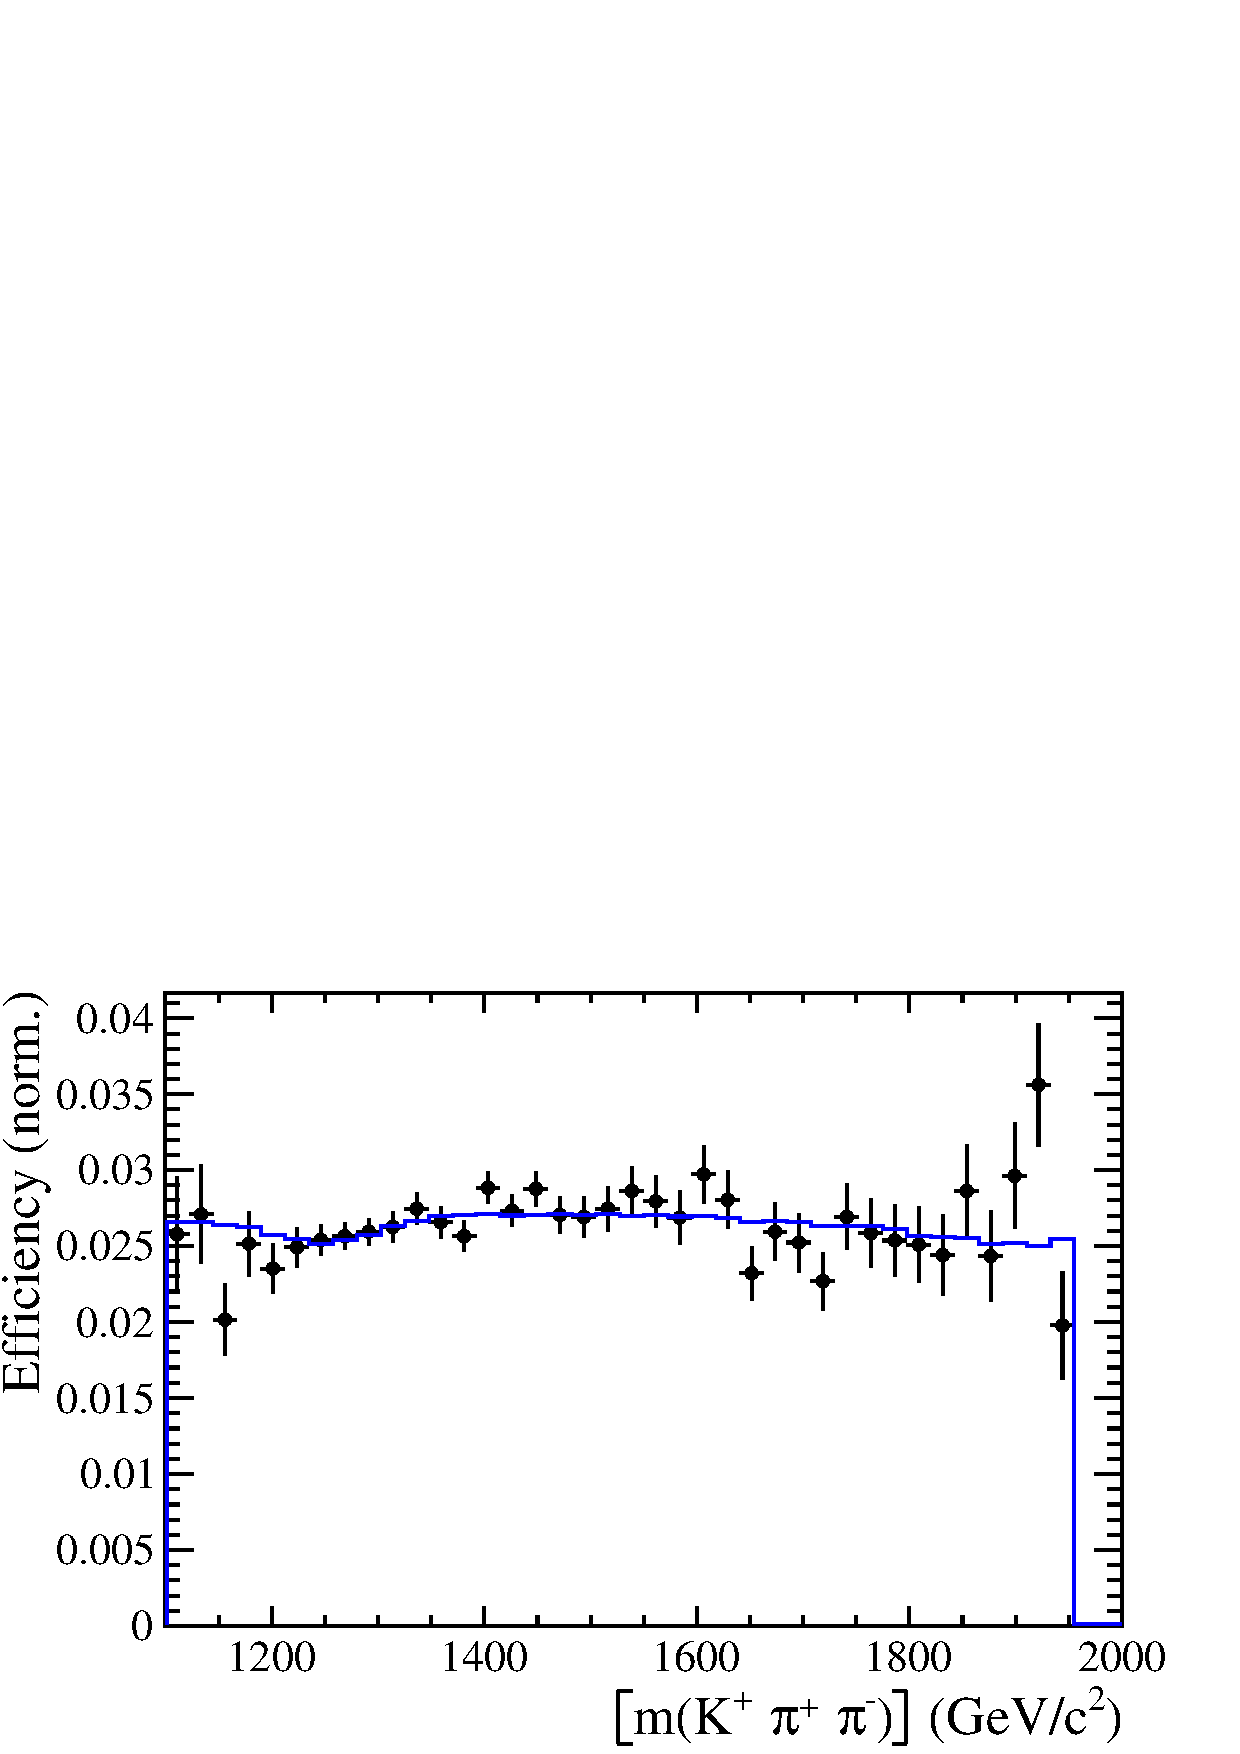
\includegraphics[height=!,width=0.4\textwidth]{figs/AcceptancePhsp/eff_Kpipi.pdf}
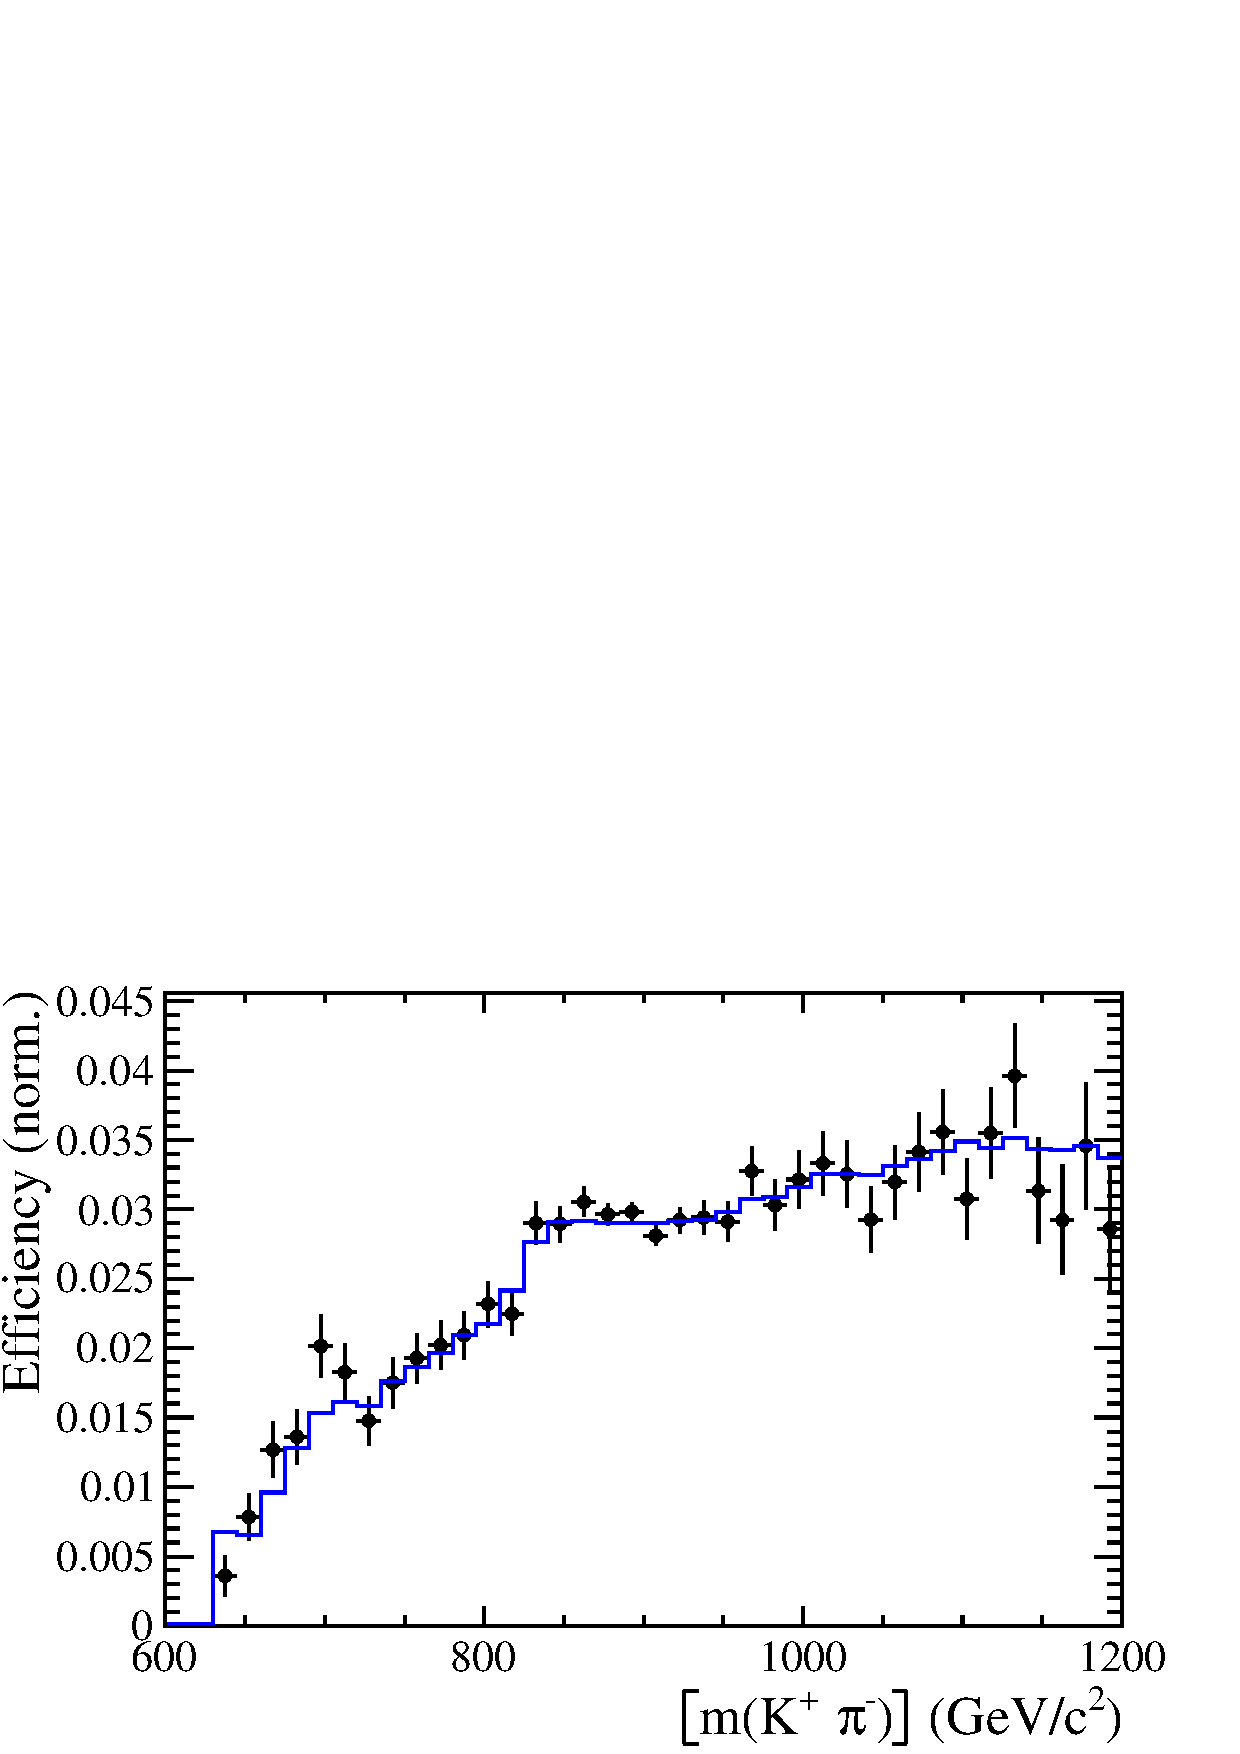
\includegraphics[height=!,width=0.4\textwidth]{figs/AcceptancePhsp/eff_Kpi.pdf}

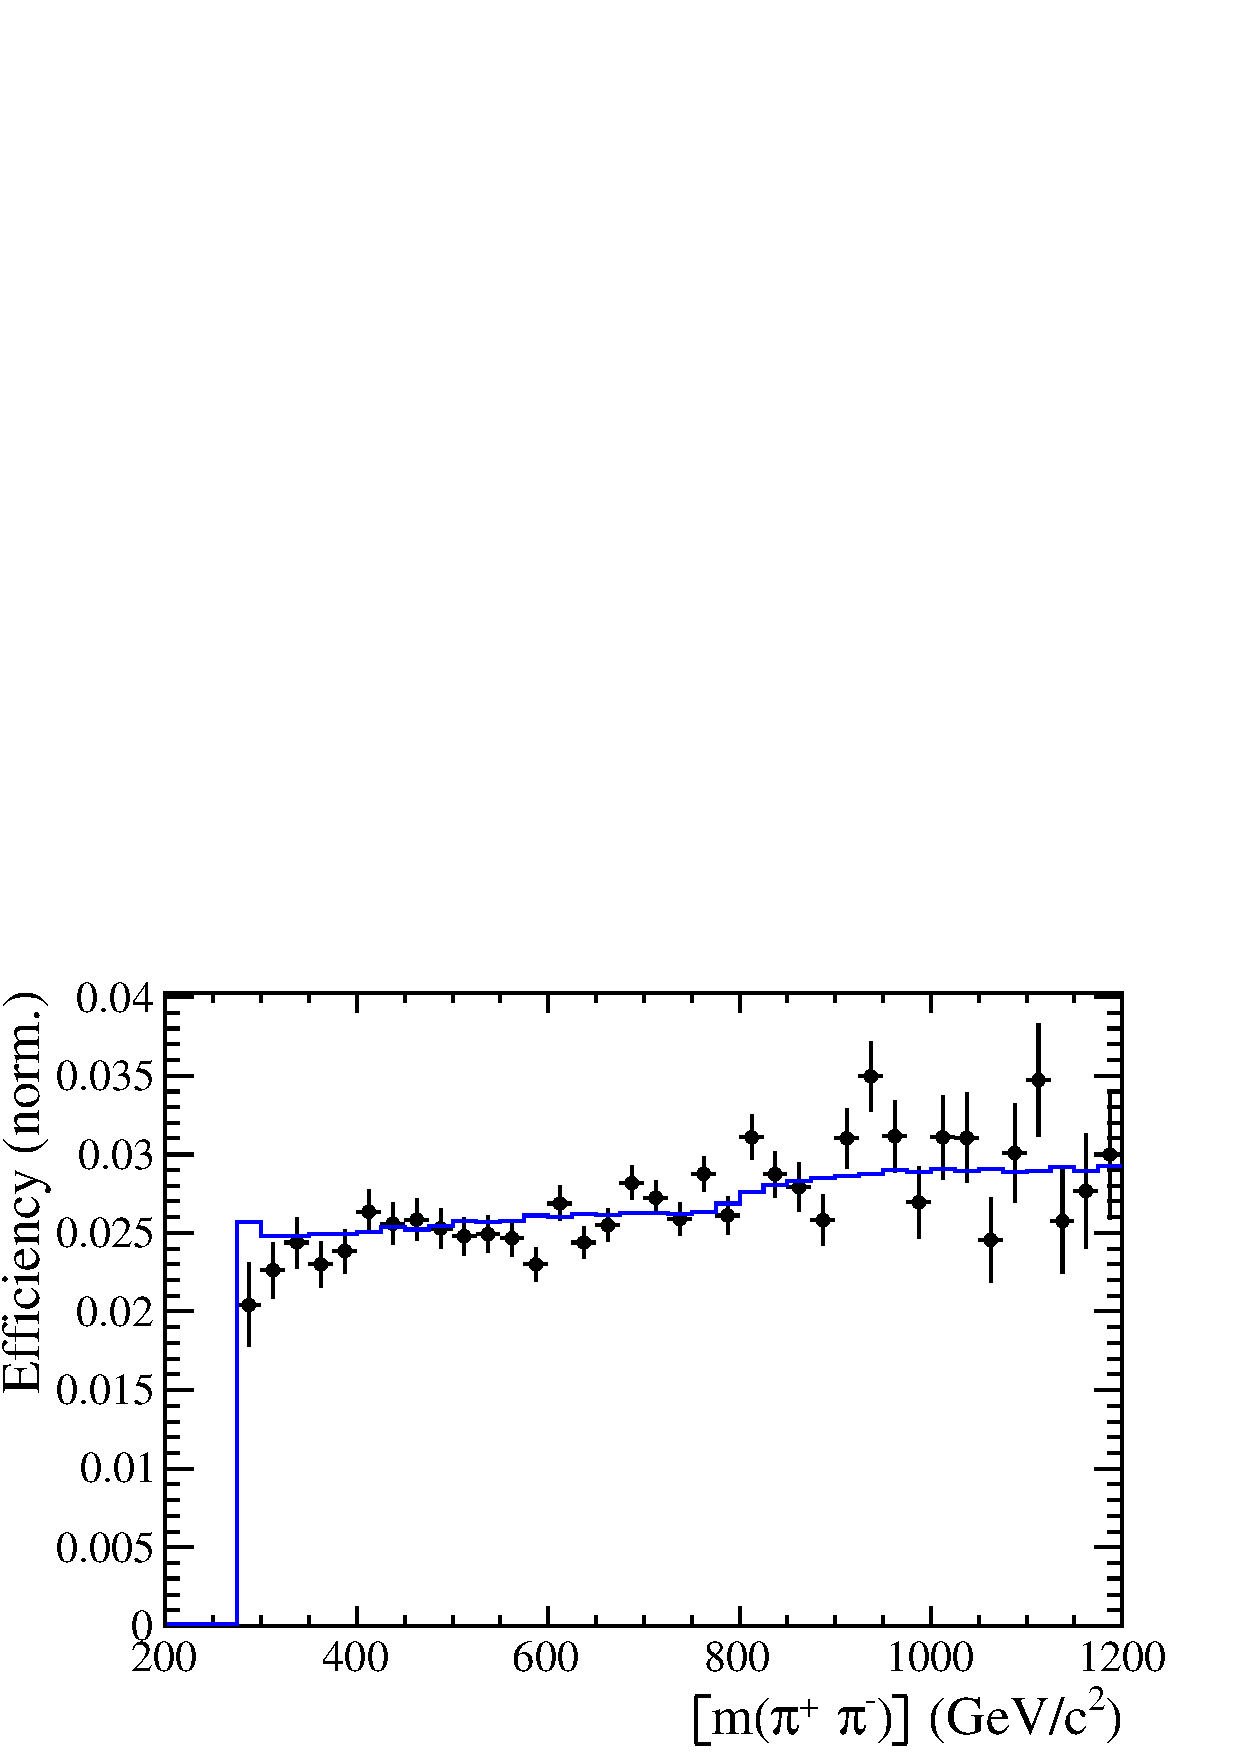
\includegraphics[height=!,width=0.4\textwidth]{figs/AcceptancePhsp/eff_pipi.pdf}
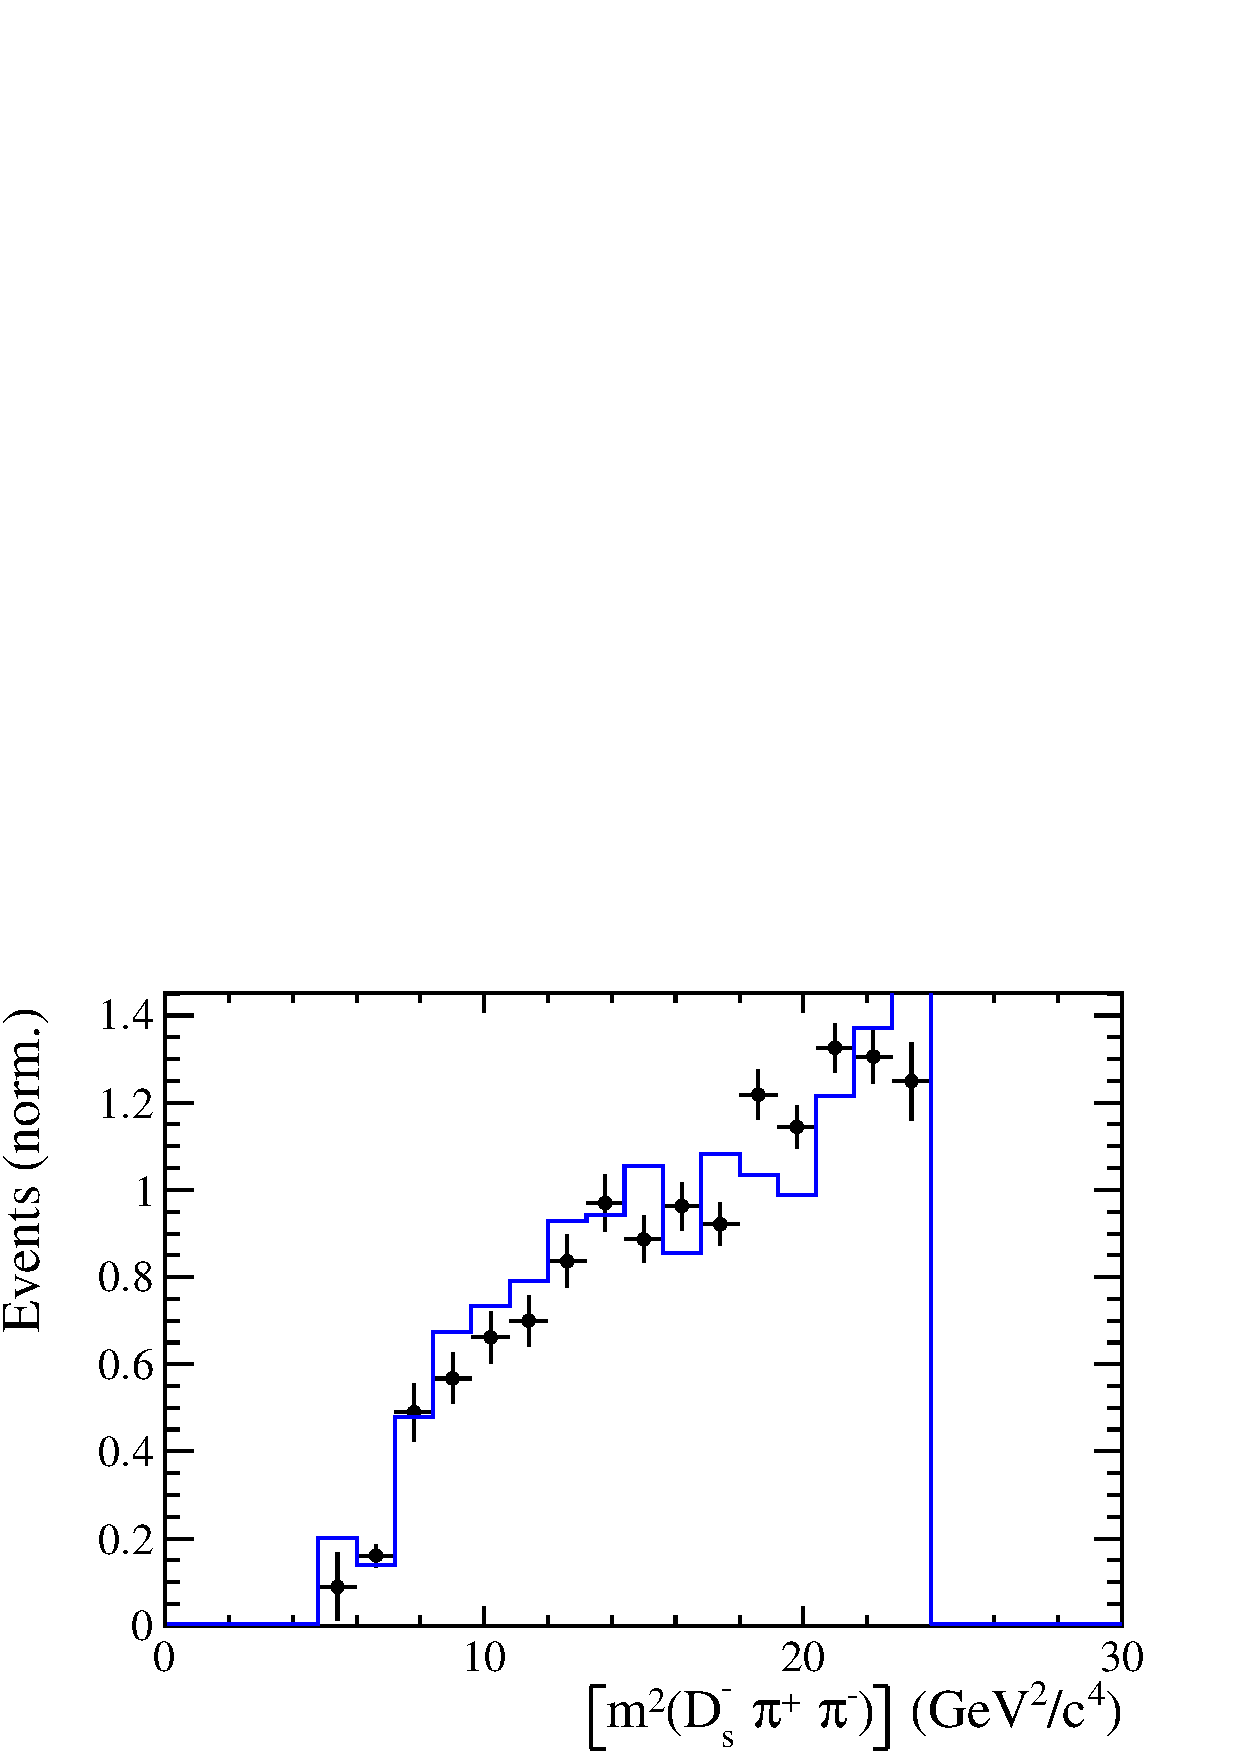
\includegraphics[height=!,width=0.4\textwidth]{figs/AcceptancePhsp/eff_Dspipi.pdf}

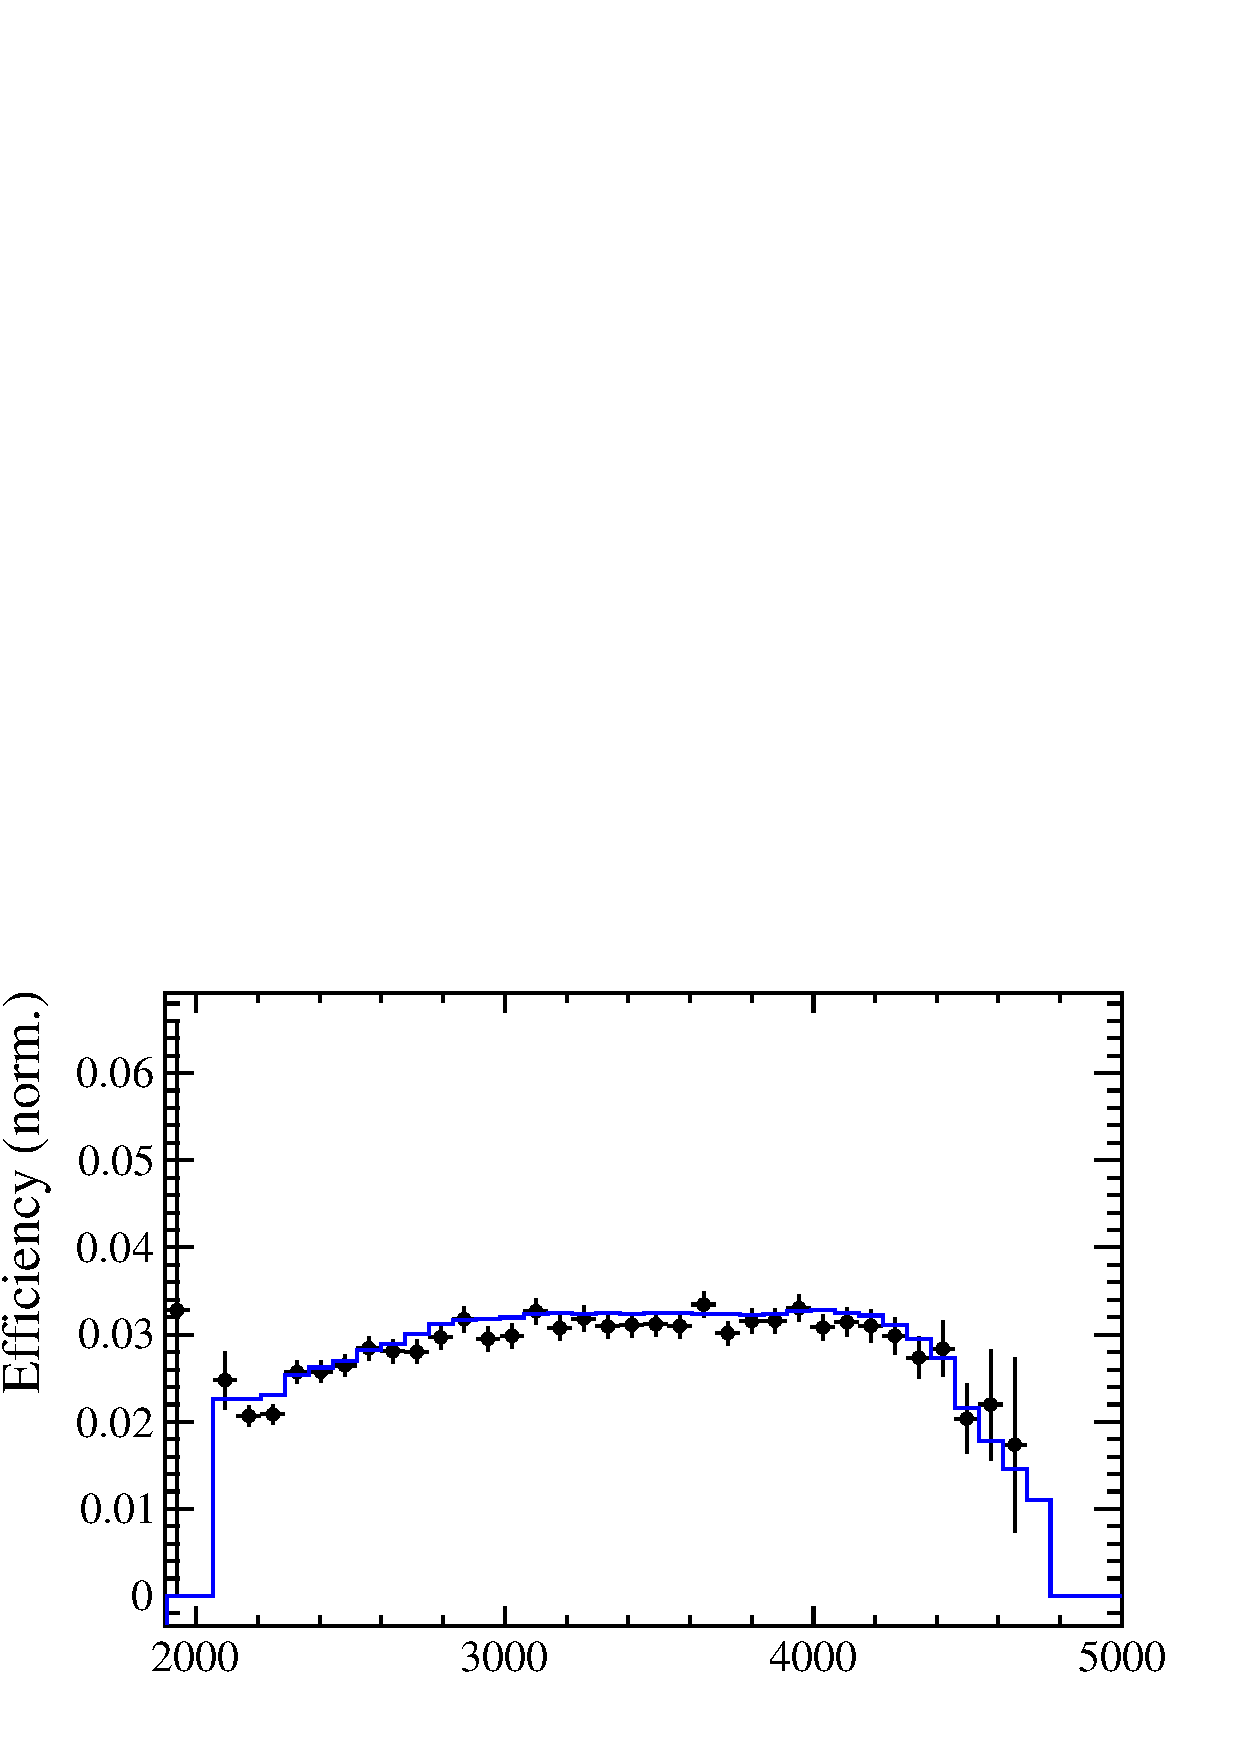
\includegraphics[height=!,width=0.4\textwidth]{figs/AcceptancePhsp/eff_Dspi.pdf}
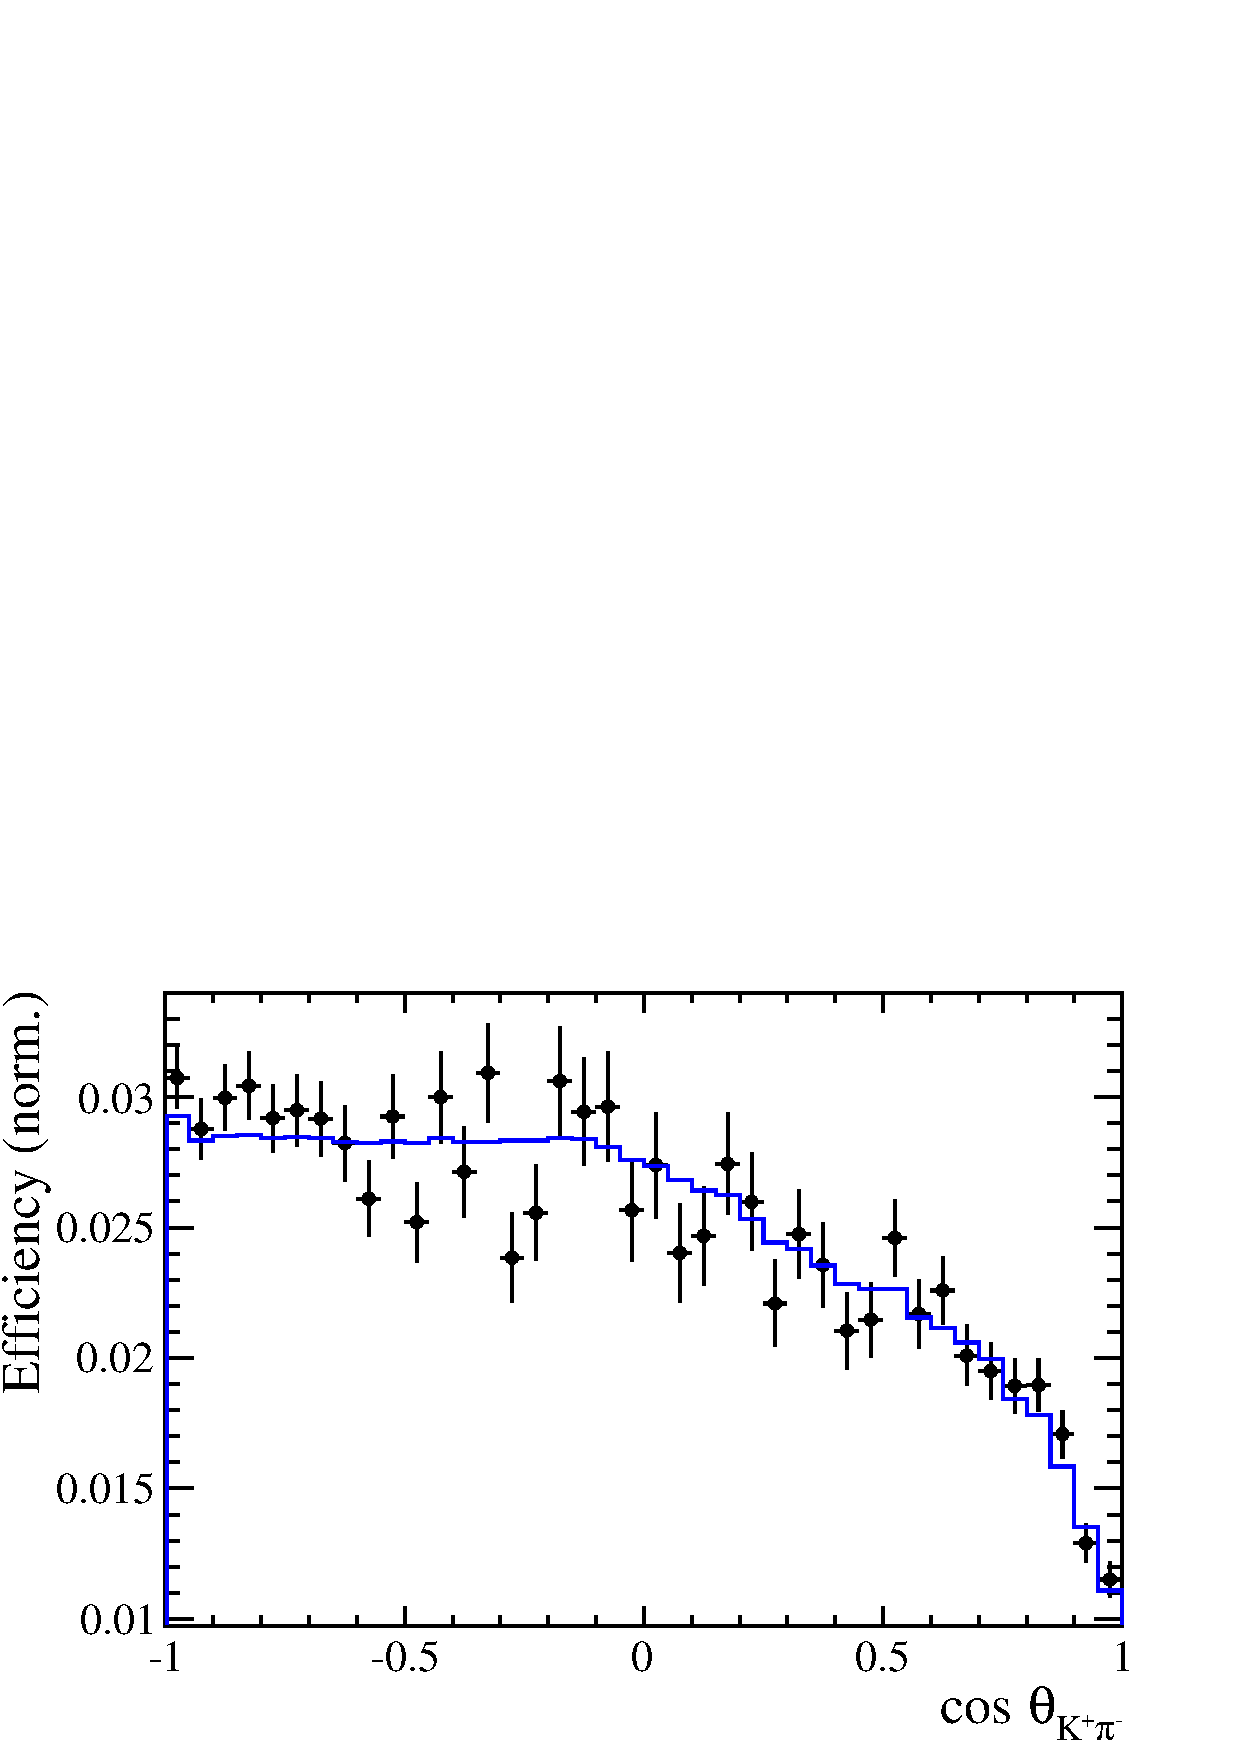
\includegraphics[height=!,width=0.4\textwidth]{figs/AcceptancePhsp/eff_cosTheta_Kpi.pdf}

\includegraphics[height=!,width=0.4\textwidth]{figs/AcceptancePhsp/eff_cosTheta_Dspi.pdf}
\includegraphics[height=!,width=0.4\textwidth]{figs/AcceptancePhsp/eff_phi_Kpi_Dspi.pdf}

\caption{Efficiency variation as a function of the phase-space variables obtained from the ratio of selected and generated MC events.
}
\label{fig:PhspEff}
\end{figure}
